\documentclass[11pt]{article}
\usepackage[margin=1in]{geometry}
\usepackage{booktabs}
\usepackage{array}
\usepackage{longtable}
\usepackage{amsmath}
\usepackage{graphicx}
\usepackage{caption}
\usepackage{float}
\usepackage[table]{xcolor}
\usepackage{tikz}
\usetikzlibrary{arrows.meta,positioning,backgrounds,fit}
\usepackage[hidelinks]{hyperref}
\definecolor{vgreen}{HTML}{1B7837}
\definecolor{vorange}{HTML}{C97A0A}
\definecolor{vred}{HTML}{C0392B}
\definecolor{vgray}{HTML}{555555}
\definecolor{fd1c}{HTML}{1f77b4}
\definecolor{fd3c}{HTML}{C0392B}
\newcommand{\ttt}[1]{\texttt{#1}}
\newcommand{\verd}[2]{\textcolor{#1}{\textbf{#2}}}
\setlength{\parindent}{0pt}
\setlength{\parskip}{0.55em}


\begin{document}

\title{\textbf{Connectomic identification, with confidence, and the full circuit of the FD2 figure-detection cell (\ttt{LPT21})}}

\author{Stage 11 FD2 Identification}

\date{\today}

\maketitle

\tableofcontents

\part{Identity: FD2 is \texttt{LPT21}}

\textbf{Summary.}\quad Egelhaaf defined FD2 as a regressive, frontal, small-field figure-detection cell that is a homolateral output element projecting to the ipsilateral posterior optic foci, with a second axonal branch running frontally toward the anterior optic foci. This report identifies the FlyWire cell type \textbf{\ttt{LPT21}} as the connectomic correlate of that FD2 phenotype and traces its complete circuit from photoreceptor input to motor output. \ttt{LPT21} draws 98.47\% of its T4/T5 motion input from the back-to-front lobula-plate layer, has a receptive field co-located with the frontal FD1 cell, sends 1.58\% of its output across the midline (a homolateral, ipsilateral projection), is cholinergic, and has two spatially separated output terminal fields matching Egelhaaf's description of a main and a frontal axonal branch. Among the lobula-plate tangential cells it is the unique full FD2 match. The identification carries a decomposed confidence of 0.88 (plausible range [0.76, 0.95]), after discounting for the absence of an independent FD2 anchor and for FD2's large-field organisation, which Egelhaaf could not resolve.

\section{Introduction}

\textbf{Figure-ground discrimination and the FD cells.}\quad
A textured object is invisible against a matched background until it moves at a different velocity or
phase; relative motion then makes it salient. Reichardt and Poggio showed behaviourally that flies
detect and track such figures~\cite{rp1979}. Egelhaaf, in a three-part study, described a class of
lobula-plate tangential cells, the figure-detection (FD) cells, each more sensitive to a small moving
figure than to wide-field motion~\cite{egelhaaf1985b}. Four were distinguished by preferred direction
and receptive-field organisation. \textbf{FD2} is excited by regressive (back-to-front) motion; its
excitatory receptive field is frontal, with its maximum at azimuth $0$--$10^\circ$ and its frontal
boundary at the margin of the ipsilateral eye, reaching laterally to about $60^\circ$ and covering the
whole vertical extent~\cite[p.~201]{egelhaaf1985b}. Anatomically FD2 is a homolateral output element
of the lobula plate: its dendrite covers the lateral lobula plate along the full dorso-ventral axis,
its main axon projects to the ipsilateral posterior optic foci, and a second branch runs frontally
for some $70$--$90\,\mu$m toward the anterior optic foci. FD2 was the least thoroughly recorded of the
FD cells, and its large-field inhibitory input could not be resolved~\cite[p.~201--202]{egelhaaf1985b}.

\textbf{The connectome era and the mapping problem.}\quad
The adult \emph{Drosophila} FlyWire connectome and its cell-type annotations provide the
synapse-resolution wiring needed to ask which modern cell type corresponds to each FD
cell~\cite{dorkenwald2024,schlegel2024,codex}. T4 and T5 encode ON/OFF edge motion and segregate by
preferred direction into the four lobula-plate layers~\cite{maisak2013,fd1989}: layer-a front-to-back,
layer-b back-to-front. FD1 has been mapped to \ttt{Nod1} and FD3 to \ttt{LPT42\_Nod4}. This report
asks which cell type is FD2, attaches a quantified confidence, and traces the cell's full circuit.

\textbf{How the identification is made.}\quad
Each defining FD2 property corresponds to a connectome measurement: preferred direction from the
lobula-plate layer of its T4/T5 input, the receptive field from the retinotopic positions of those
inputs relative to the frontal FD1 cell, the projection side from where its output synapses land, the
dual axonal output from the spatial distribution of those synapses, and overall shape from its
reconstructed skeleton. We measure each for \ttt{LPT21}, compare against a global scan of the
lobula-plate tangential family so uniqueness is measured rather than assumed, and combine the results
into a transparent confidence interval. Figure~\ref{fig:concept} fixes the FD2 phenotype.

\begin{figure}[H]\centering
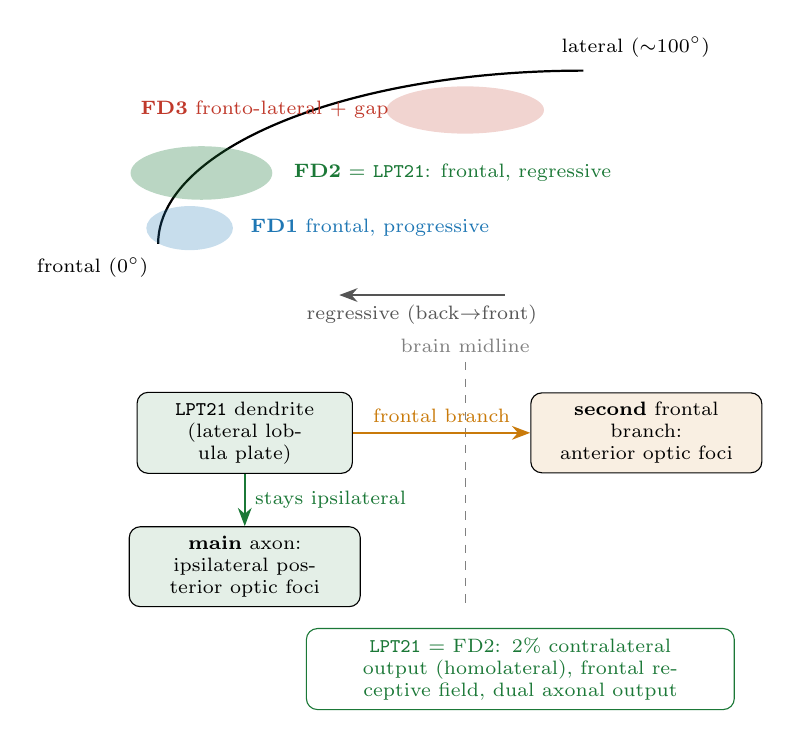
\begin{tikzpicture}[font=\small,>=Stealth]
  \draw[thick] (0,0) arc (180:90:5.4 and 2.2);
  \node[anchor=north east,font=\scriptsize] at (0,-0.05) {frontal ($0^\circ$)};
  \node[anchor=south west,font=\scriptsize] at (5.0,2.25) {lateral ($\sim$100$^\circ$)};
  % FD1 frontal (progressive) anchor
  \fill[fd1c,opacity=0.25] (0.4,0.2) ellipse (0.55 and 0.28);
  \node[fd1c,font=\scriptsize,anchor=west] at (1.05,0.2) {\textbf{FD1} frontal, progressive};
  % FD2 = LPT21: frontal, regressive, homolateral
  \fill[vgreen,opacity=0.30] (0.55,0.9) ellipse (0.9 and 0.34);
  \node[vgreen,font=\scriptsize,anchor=west] at (1.6,0.9) {\textbf{FD2} $=$ \ttt{LPT21}: frontal, regressive};
  % FD3 fronto-lateral + gap (context)
  \fill[fd3c,opacity=0.22] (3.9,1.7) ellipse (1.0 and 0.30);
  \node[fd3c,font=\scriptsize,anchor=east] at (3.05,1.7) {\textbf{FD3} fronto-lateral $+$ gap};
  \draw[->,thick,vgray] (4.4,-0.65) -- (2.3,-0.65)
        node[midway,below,font=\scriptsize]{regressive (back$\to$front)};
  % projection: FD2 axon stays ipsilateral (homolateral), with a frontal branch
  \draw[dashed,gray] (3.9,-1.5) -- (3.9,-4.6);
  \node[gray,font=\scriptsize,anchor=south] at (3.9,-1.5) {brain midline};
  \node[draw,rounded corners,fill=vgreen!12,font=\scriptsize,align=center,text width=2.5cm]
        (d) at (1.1,-2.4) {\ttt{LPT21} dendrite\\(lateral lobula plate)};
  \node[draw,rounded corners,fill=vgreen!12,font=\scriptsize,align=center,text width=2.7cm]
        (a1) at (1.1,-4.1) {\textbf{main} axon:\\ipsilateral posterior optic foci};
  \node[draw,rounded corners,fill=vorange!12,font=\scriptsize,align=center,text width=2.7cm]
        (a2) at (6.2,-2.4) {\textbf{second} frontal branch:\\anterior optic foci};
  \draw[->,thick,vgreen] (d) -- node[right,font=\scriptsize]{stays ipsilateral} (a1);
  \draw[->,thick,vorange] (d) -- node[above,midway,font=\scriptsize]{frontal branch} (a2);
  \node[draw,rounded corners,vgreen,font=\scriptsize,align=center,text width=5.2cm]
        at (4.6,-5.4) {\ttt{LPT21} $=$ FD2: 2\% contralateral output (homolateral), frontal receptive field, dual axonal output};
\end{tikzpicture}
\caption{\textbf{The FD2 cell and what distinguishes it.} Egelhaaf (1985, Part II) described FD2 as a
regressive figure-detection cell with a frontal receptive field reaching the frontal margin of the
ipsilateral eye, and as a homolateral output element whose main axon projects to the ipsilateral
posterior optic foci with a second branch running frontally toward the anterior optic foci. It is the
frontal, regressive member of the FD set (FD1 is frontal and progressive; FD3 is fronto-lateral with a
frontal gap and a contralateral axon). This report maps FD2 onto the FlyWire cell type \ttt{LPT21}.}%
\label{fig:concept}
\end{figure}


\section{The evidence}

We take FD2's defining properties in turn: preferred motion, receptive field, projection side, small-field selectivity, transmitter, and the dual axonal output.

\paragraph{It prefers back-to-front motion.} A cell's preferred direction is read from which lobula-plate layer its motion inputs come from. For \ttt{LPT21}, 98.47\% of that input comes from the back-to-front layer (Fig.~\ref{fig:census}b), the regressive direction Egelhaaf reported for FD2.

\paragraph{Its receptive field is frontal.} Measured against the frontal FD1 cell in the same coordinate frame, the input field of \ttt{LPT21} sits at the FD1 position (offset near zero, about 0.07 lattice columns) and fills the frontal band on both sides, the frontal receptive field Egelhaaf described for FD2 reaching the margin of the ipsilateral eye (Fig.~\ref{fig:hexmap}).

\paragraph{Its axon stays on its own side of the brain.} Egelhaaf found that FD2 is a homolateral cell whose main axon projects to the ipsilateral posterior optic foci. The connectome shows the same: 1.58\% of \ttt{LPT21}'s output synapses are on the opposite side of the brain, that is, almost all of its output stays ipsilateral. This is the homolateral projection of FD2, and it is the property that separates FD2 from the contralaterally projecting FD3.

\paragraph{It responds to small objects.} The defining behaviour of an FD cell is a stronger response to a small moving figure than to wide-field motion, which requires the cell to pool a compact patch of the visual field. The input patch of \ttt{LPT21} is more concentrated than an in-degree matched random sample ($p=0.002$). This provides wiring support for small-field selectivity.

\paragraph{It is an excitatory output cell.} \ttt{LPT21} is a bilateral pair classified as a visual output neuron, releasing the excitatory transmitter acetylcholine (confidence 0.8132). Egelhaaf did not report the transmitter of FD2; this is a connectome assignment.

\paragraph{It has two separate axonal outputs.} Egelhaaf reported that FD2 alone among the FD cells has a second axonal branch, running frontally toward the anterior optic foci, and proposed it may drive the landing response. The connectome shows the same: the output synapses of each \ttt{LPT21} cell form two spatially separated terminal fields (bimodal on both cells: True), a main field and a smaller displaced field, matching the two axonal branches Egelhaaf described (Fig.~\ref{fig:dual}).

\begin{figure}[H]\centering
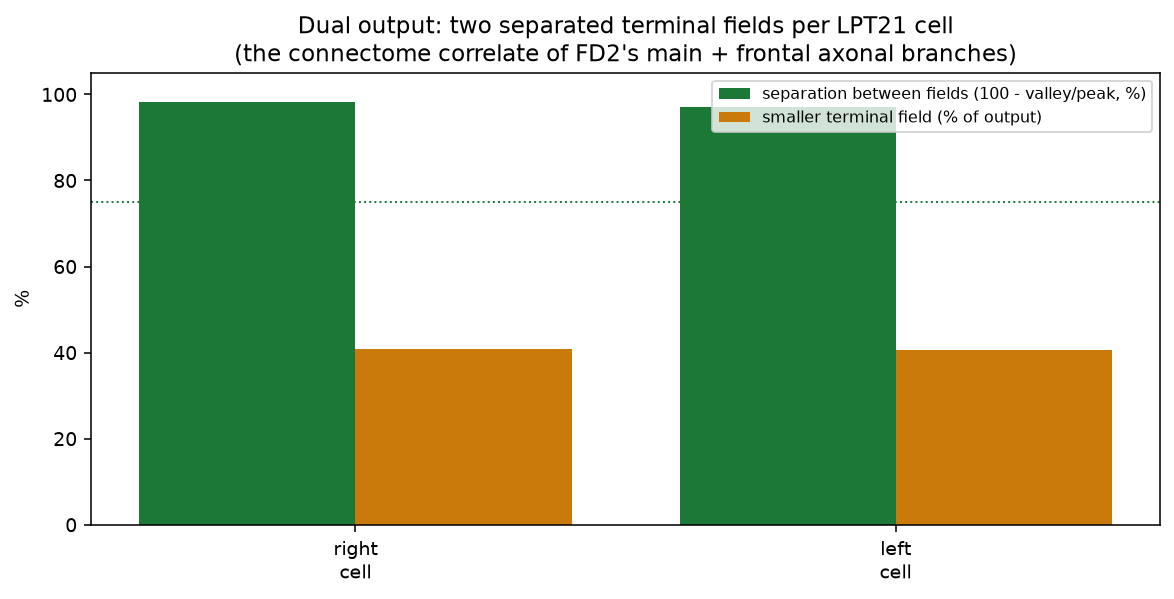
\includegraphics[width=\textwidth]{figures/fd2_dual_output.png}
\caption{\textbf{The dual output.} For each \ttt{LPT21} cell, the separation between its two output terminal fields (measured as the depth of the valley between them) and the size of the smaller field. Two well-separated fields per cell are the connectome correlate of Egelhaaf's main (ipsilateral posterior optic foci) and second (frontal, anterior optic foci) axonal branches.}\label{fig:dual}
\end{figure}


\begin{figure}[H]\centering
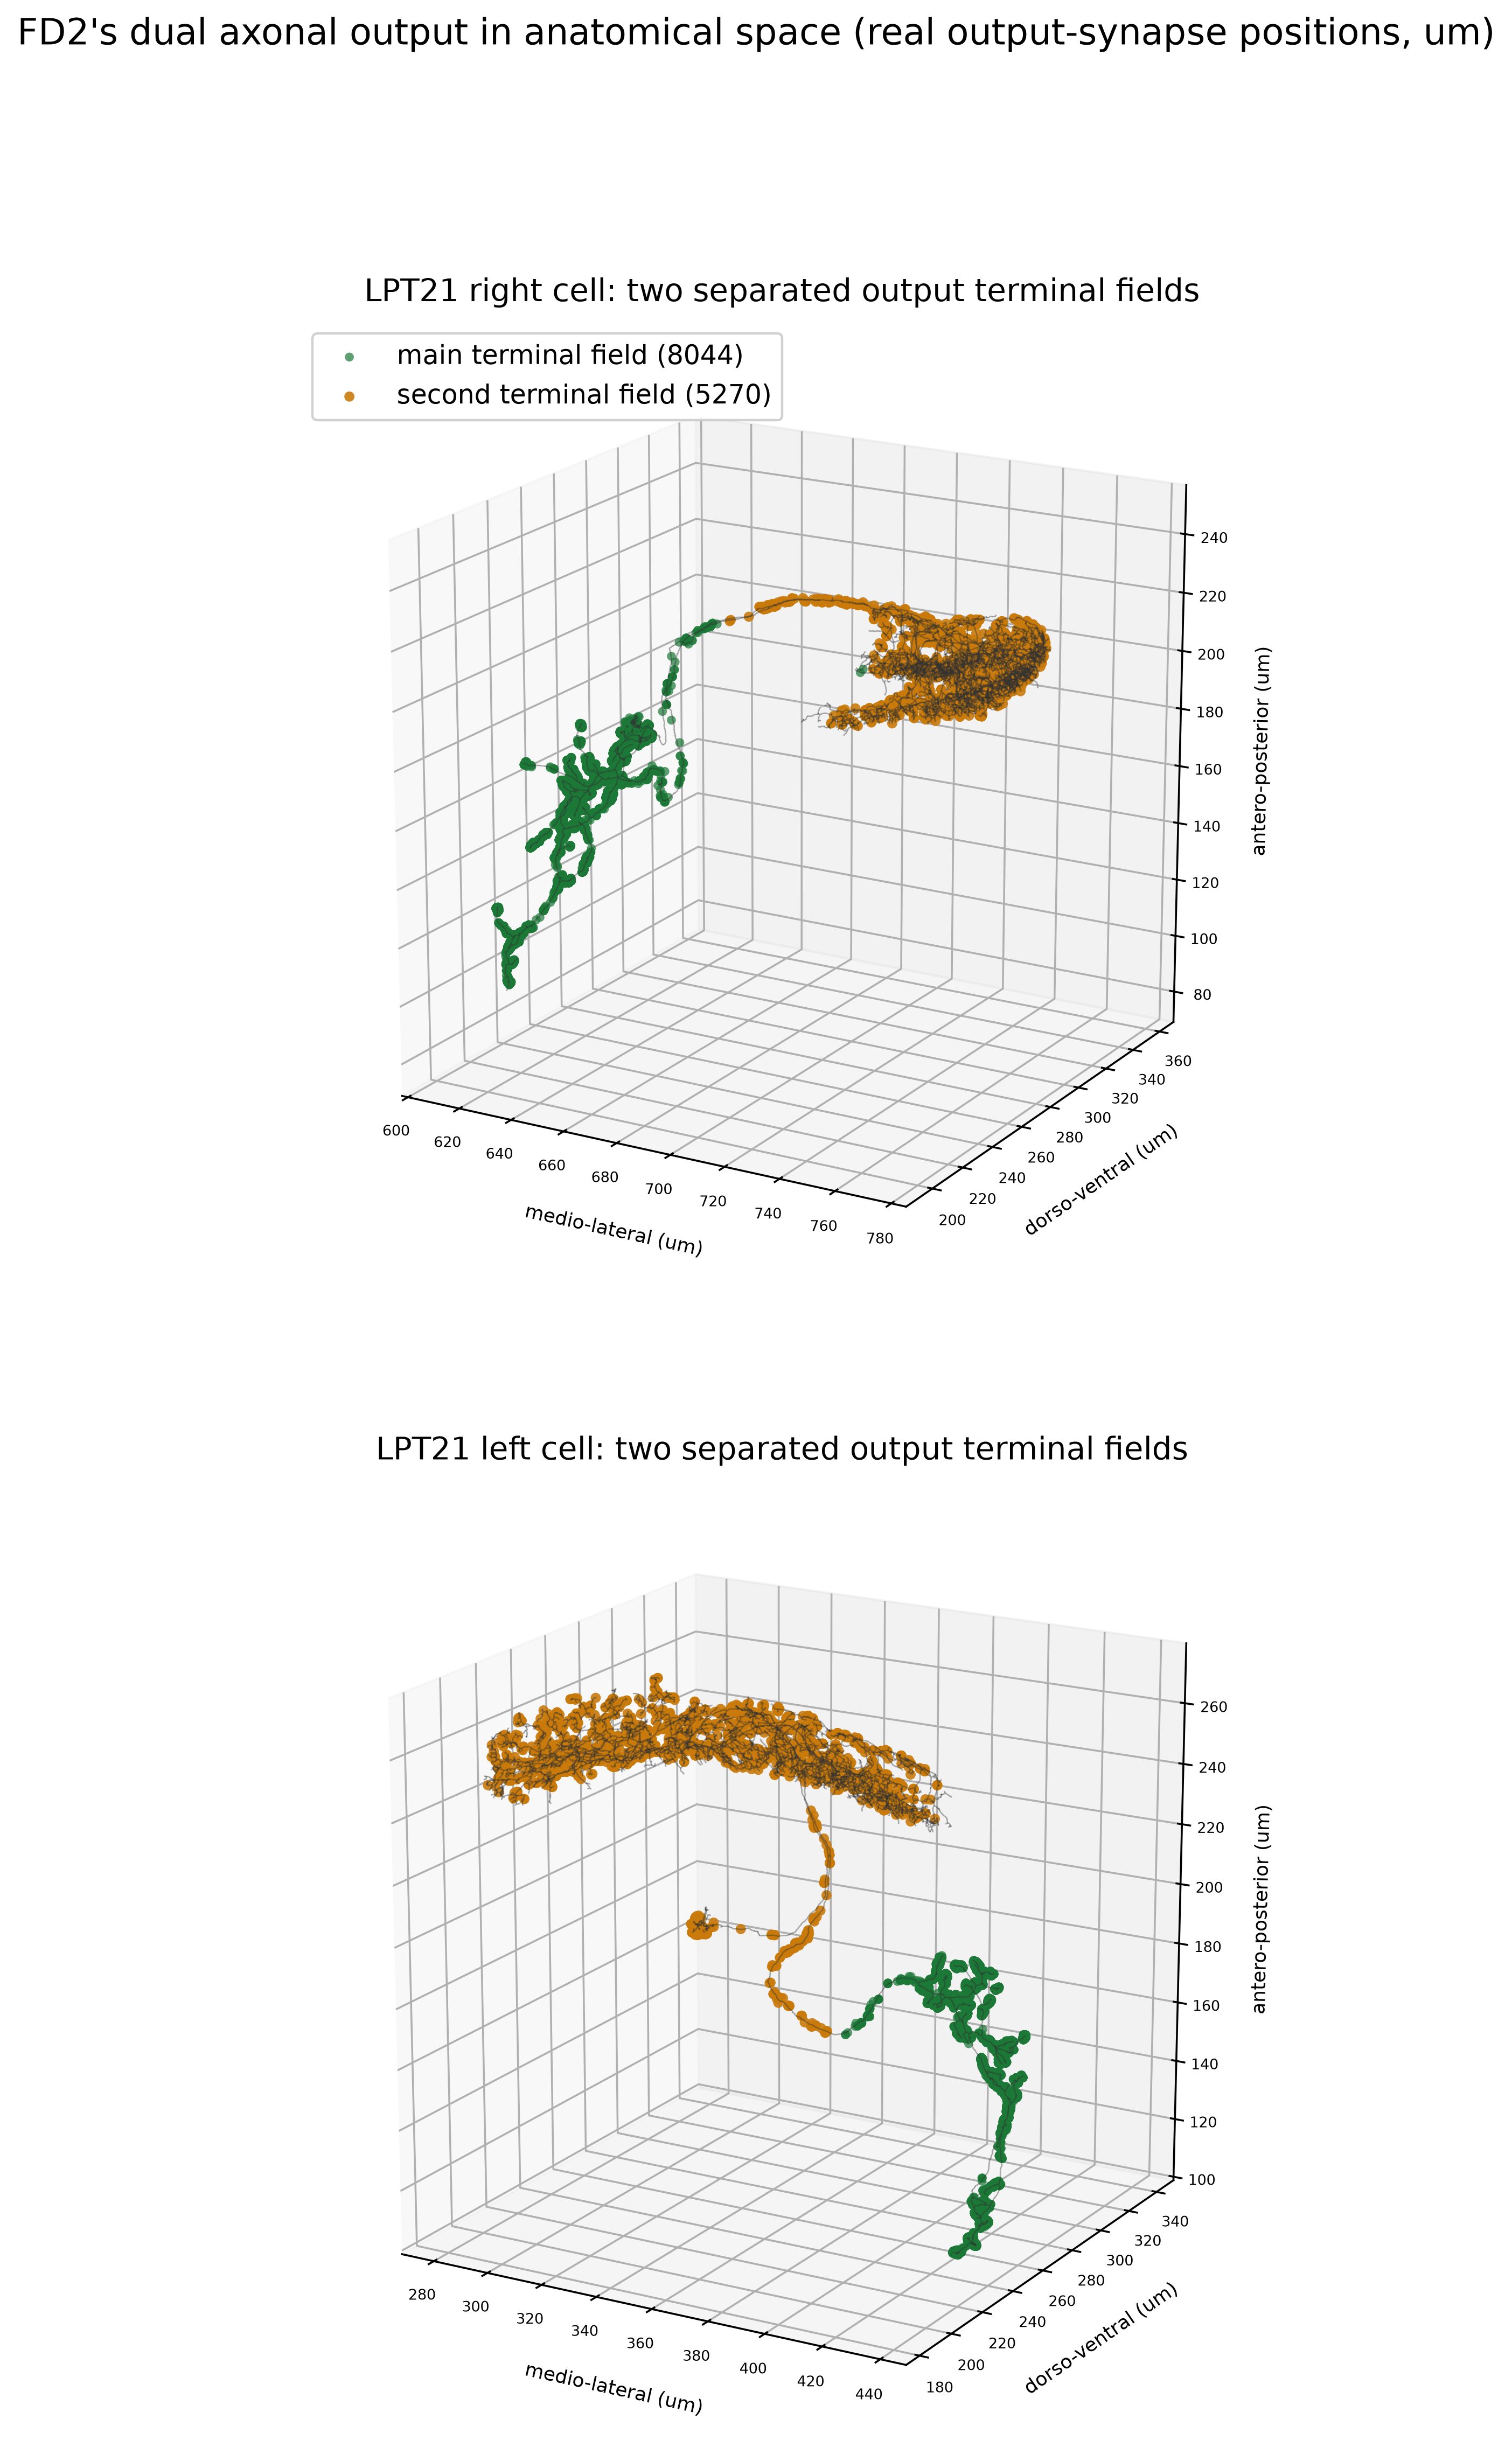
\includegraphics[width=\textwidth]{figures/fd2_dual_output_3d.png}
\caption{\textbf{The dual output in anatomical space.} The output synapses of each \ttt{LPT21} cell, coloured by which of the two terminal fields they fall in, on the reconstructed cell. The two spatially separated fields are directly visible, confirming the second axonal branch Egelhaaf described.}\label{fig:dual3d}
\end{figure}


\section{Confidence in the identification}

The identification is expressed as a decomposed confidence rather than an assertion. It combines three factors, each stated so a reader can reconstruct it. First, the fraction of FD2-defining properties \ttt{LPT21} matches: 6 of 6 (Fig.~\ref{fig:confidence}, left). Second, a global scan of the lobula-plate tangential family for cells that satisfy the whole FD2 conjunction (regressive, cholinergic, homolateral, a single bilateral pair, and a bilaterally consistent frontal field): \ttt{LPT21} is the unique full match (1 hit(s); Fig.~\ref{fig:uniqueness}). The only other regressive homolateral cholinergic cell, \ttt{LPT23}, is excluded because it is not a single bilateral pair and its receptive field is not the homogeneous frontal field of FD2. Third, explicit discounts cap the estimate: FD2 has no independent connectome anchor of the kind that fixes FD1 to \ttt{Nod1}, so the identity is an inference from property consistency and uniqueness; Egelhaaf could not resolve FD2's large-field organisation, so that axis cannot corroborate; further undiscovered FD cells cannot be excluded; and the cell is a single bilateral pair. The resulting point estimate is 0.88, with a plausible range of [0.76, 0.95].

\begin{figure}[H]\centering
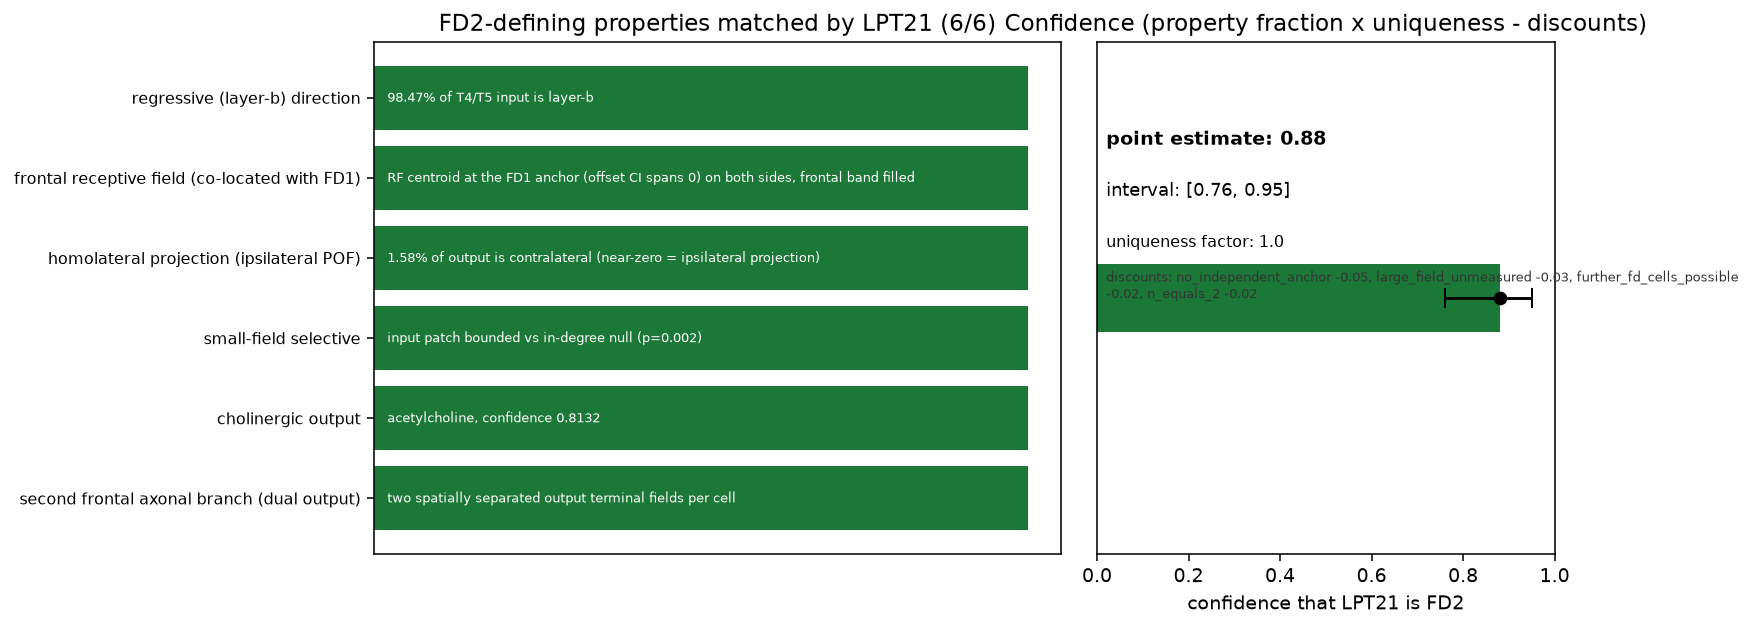
\includegraphics[width=\textwidth]{figures/fd2_confidence.png}
\caption{\textbf{The confidence, decomposed.} (left) The FD2-defining properties and whether \ttt{LPT21} matches each. (right) The point estimate and interval, with the uniqueness factor and the discounts that set it.}\label{fig:confidence}
\end{figure}
\begin{figure}[H]\centering
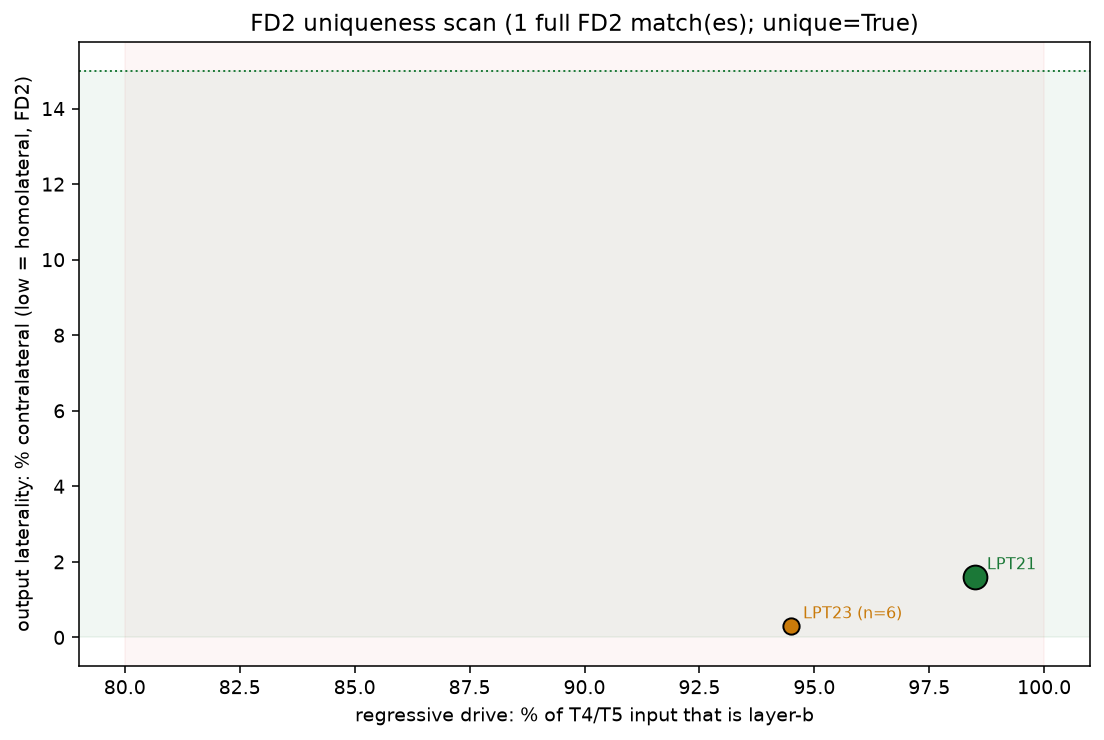
\includegraphics[width=\textwidth]{figures/fd2_uniqueness.png}
\caption{\textbf{The uniqueness scan.} Every scanned lobula-plate tangential cell placed by its regressive drive (horizontal) and output laterality (vertical). \ttt{LPT21} occupies the FD2 corner (regressive and homolateral); any cell sharing the corner is labelled with why it is not FD2.}\label{fig:uniqueness}
\end{figure}


\section{The evidence at a glance}

Table~\ref{tab:evidence} collects the defining FD2 properties next to the connectome measurement that establishes each for \ttt{LPT21}.

\begin{table}[H]\centering\footnotesize\caption{Each defining property of Egelhaaf's FD2 cell and the matching measurement for the FlyWire cell type \ttt{LPT21}.}\label{tab:evidence}

\renewcommand{\arraystretch}{1.25}
\setlength{\tabcolsep}{3pt}
\begin{longtable}{@{}>{\raggedright\arraybackslash}p{0.26\textwidth} >{\raggedright\arraybackslash}p{0.32\textwidth} >{\raggedright\arraybackslash}p{0.36\textwidth}@{}}
\toprule \textbf{FD2 property} & \textbf{What Egelhaaf reported} & \textbf{What we find for \ttt{LPT21}} \\\midrule\endhead
Prefers regressive (back-to-front) motion & Egelhaaf: FD2 excited by regressive motion & 98.47\% of its T4/T5 input is the back-to-front layer \\
Frontal receptive field & Egelhaaf: peak azimuth $0$--$10^\circ$, at the eye's frontal margin & input field co-located with the frontal FD1 cell, frontal band filled, no gap \\
Homolateral (ipsilateral) projection & Egelhaaf: main axon to the ipsilateral posterior optic foci & 1.58\% of output crosses the midline (near-zero = ipsilateral) \\
Small-object selective & FD cells prefer small figures to wide-field motion & input patch bounded below an in-degree matched null \\
Excitatory output (cholinergic) & FD cells are excitatory output neurons & acetylcholine, confidence 0.8132 \\
Second frontal axonal branch & Egelhaaf: a second branch runs frontally to the anterior optic foci & two separated output terminal fields per cell (bimodal: True) \\
Unique in the tangential family & the identification should be specific & 1 full FD2 match(es); unique: True \\
Confidence & quantify the identification honestly & point 0.88, range [0.76, 0.95] \\
\bottomrule\end{longtable}
\renewcommand{\arraystretch}{1.0}
\setlength{\tabcolsep}{6pt}

\end{table}

\section{What the data can and cannot settle}

\textbf{FD2 has no independent connectome anchor.} FD1 was fixed to \ttt{Nod1} and FD3 to \ttt{LPT42\_Nod4} before FD2 was approached, but no cell is independently known to be FD2, so this identification rests on the consistency of the measured properties with Egelhaaf's description and on the uniqueness scan, not on anchoring. The receptive-field comparison is moreover made relative to the FD1=\ttt{Nod1} cell, itself an assumed mapping, so an error in that anchor would propagate; this is one of the reasons the confidence is held below certainty. \textbf{FD2's large-fieldorganisation was never measured.} Egelhaaf could not resolve FD2's inhibitory large-field input, so that axis, resolved here from the connectome, corroborates but was not part of the physiological definition. \textbf{The cell is one bilateral pair.} Robustness comes from the left and right cell agreeing and from resampling the thousands of synapses each makes, not from a population average. \textbf{Absolute visual angle is approximate.} The receptive-field argument is built on the relative comparison to the frontal FD1 cell and does not rely on absolute azimuth. \textbf{The dual output matches FD2 but is not FD2-exclusive in the connectome.} Two separated output terminal fields match Egelhaaf's description of FD2's main and frontal branches; other tangential cells with a midline-crossing axon also show two output lobes for a different reason, so this feature corroborates the FD2 phenotype rather than proving it in isolation. \textbf{Every load-bearing claim was tested adversarially.} The identity, the motion drive, the descending output, the dual output, and the confidence interval were each subjected to an independent attempt at refutation with fresh connectome queries; each survived, and the honest residual caveats from that exercise are the ones stated here.

\clearpage

\part{Inputs: what drives FD2}

\textbf{Summary.}\quad This part follows the wiring that drives FD2 from the eye: from the photoreceptors, through the lamina and medulla, to the local motion detectors, and onto \ttt{LPT21}'s dendrite. Its measured T4/T5 motion input is 98.47\% back-to-front, carried by both the ON (\ttt{T4b}) and OFF (\ttt{T5b}) detectors, and is about 38.6\% of its total input, the rest coming from columnar projection sheets and inhibitory cells.

\section{The motion detectors that drive FD2}

Of \ttt{LPT21}'s input from the local motion detectors, 98.47\% comes from the back-to-front (layer-b) channel, carried by both the ON detector \ttt{T4b} (3597 synapses) and the OFF detector \ttt{T5b} (3562 synapses), a roughly even ON/OFF mix. FD2 therefore pools back-to-front motion of both contrast polarities (Fig.~\ref{fig:census}).

\begin{figure}[H]\centering
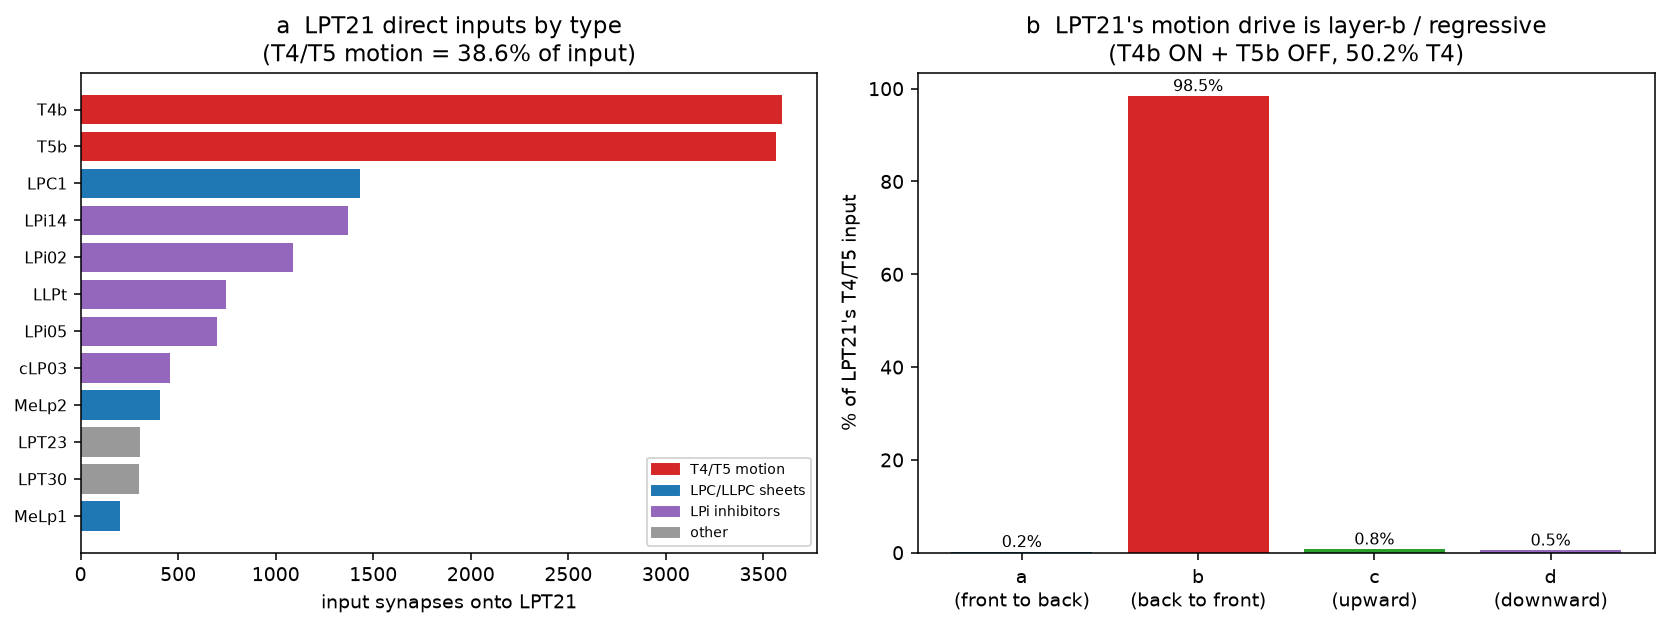
\includegraphics[width=\textwidth]{figures/fd2_input_census.png}
\caption{\textbf{What feeds FD2.} (a) \ttt{LPT21}'s direct inputs by type, coloured by class: the motion detectors, the columnar projection sheets, and the inhibitory cells. (b) Within the motion input, almost all is the back-to-front (layer-b) channel, split between the ON and OFF detectors.}\label{fig:census}
\end{figure}


\section{From the eye to the detectors}

The \ttt{T4b} cells that drive FD2 are fed by the canonical ON medulla cells and the \ttt{T5b} cells by the canonical OFF medulla cells; these are fed by the lamina and, before it, the photoreceptors. The whole cascade from the eye to FD2's detectors is present in the connectome (ON medulla present: --; OFF medulla: --; lamina: ['L1', 'L2', 'L3', 'L4', 'L5']; photoreceptors: ['R1-6', 'R7', 'R8']) and matches published optic-lobe wiring (Fig.~\ref{fig:cascade}). This cascade is the general column-to-column wiring of the optic lobe, shown as the pathway that culminates in FD2's detectors, not as a per-object trace unique to FD2.

\begin{figure}[H]\centering
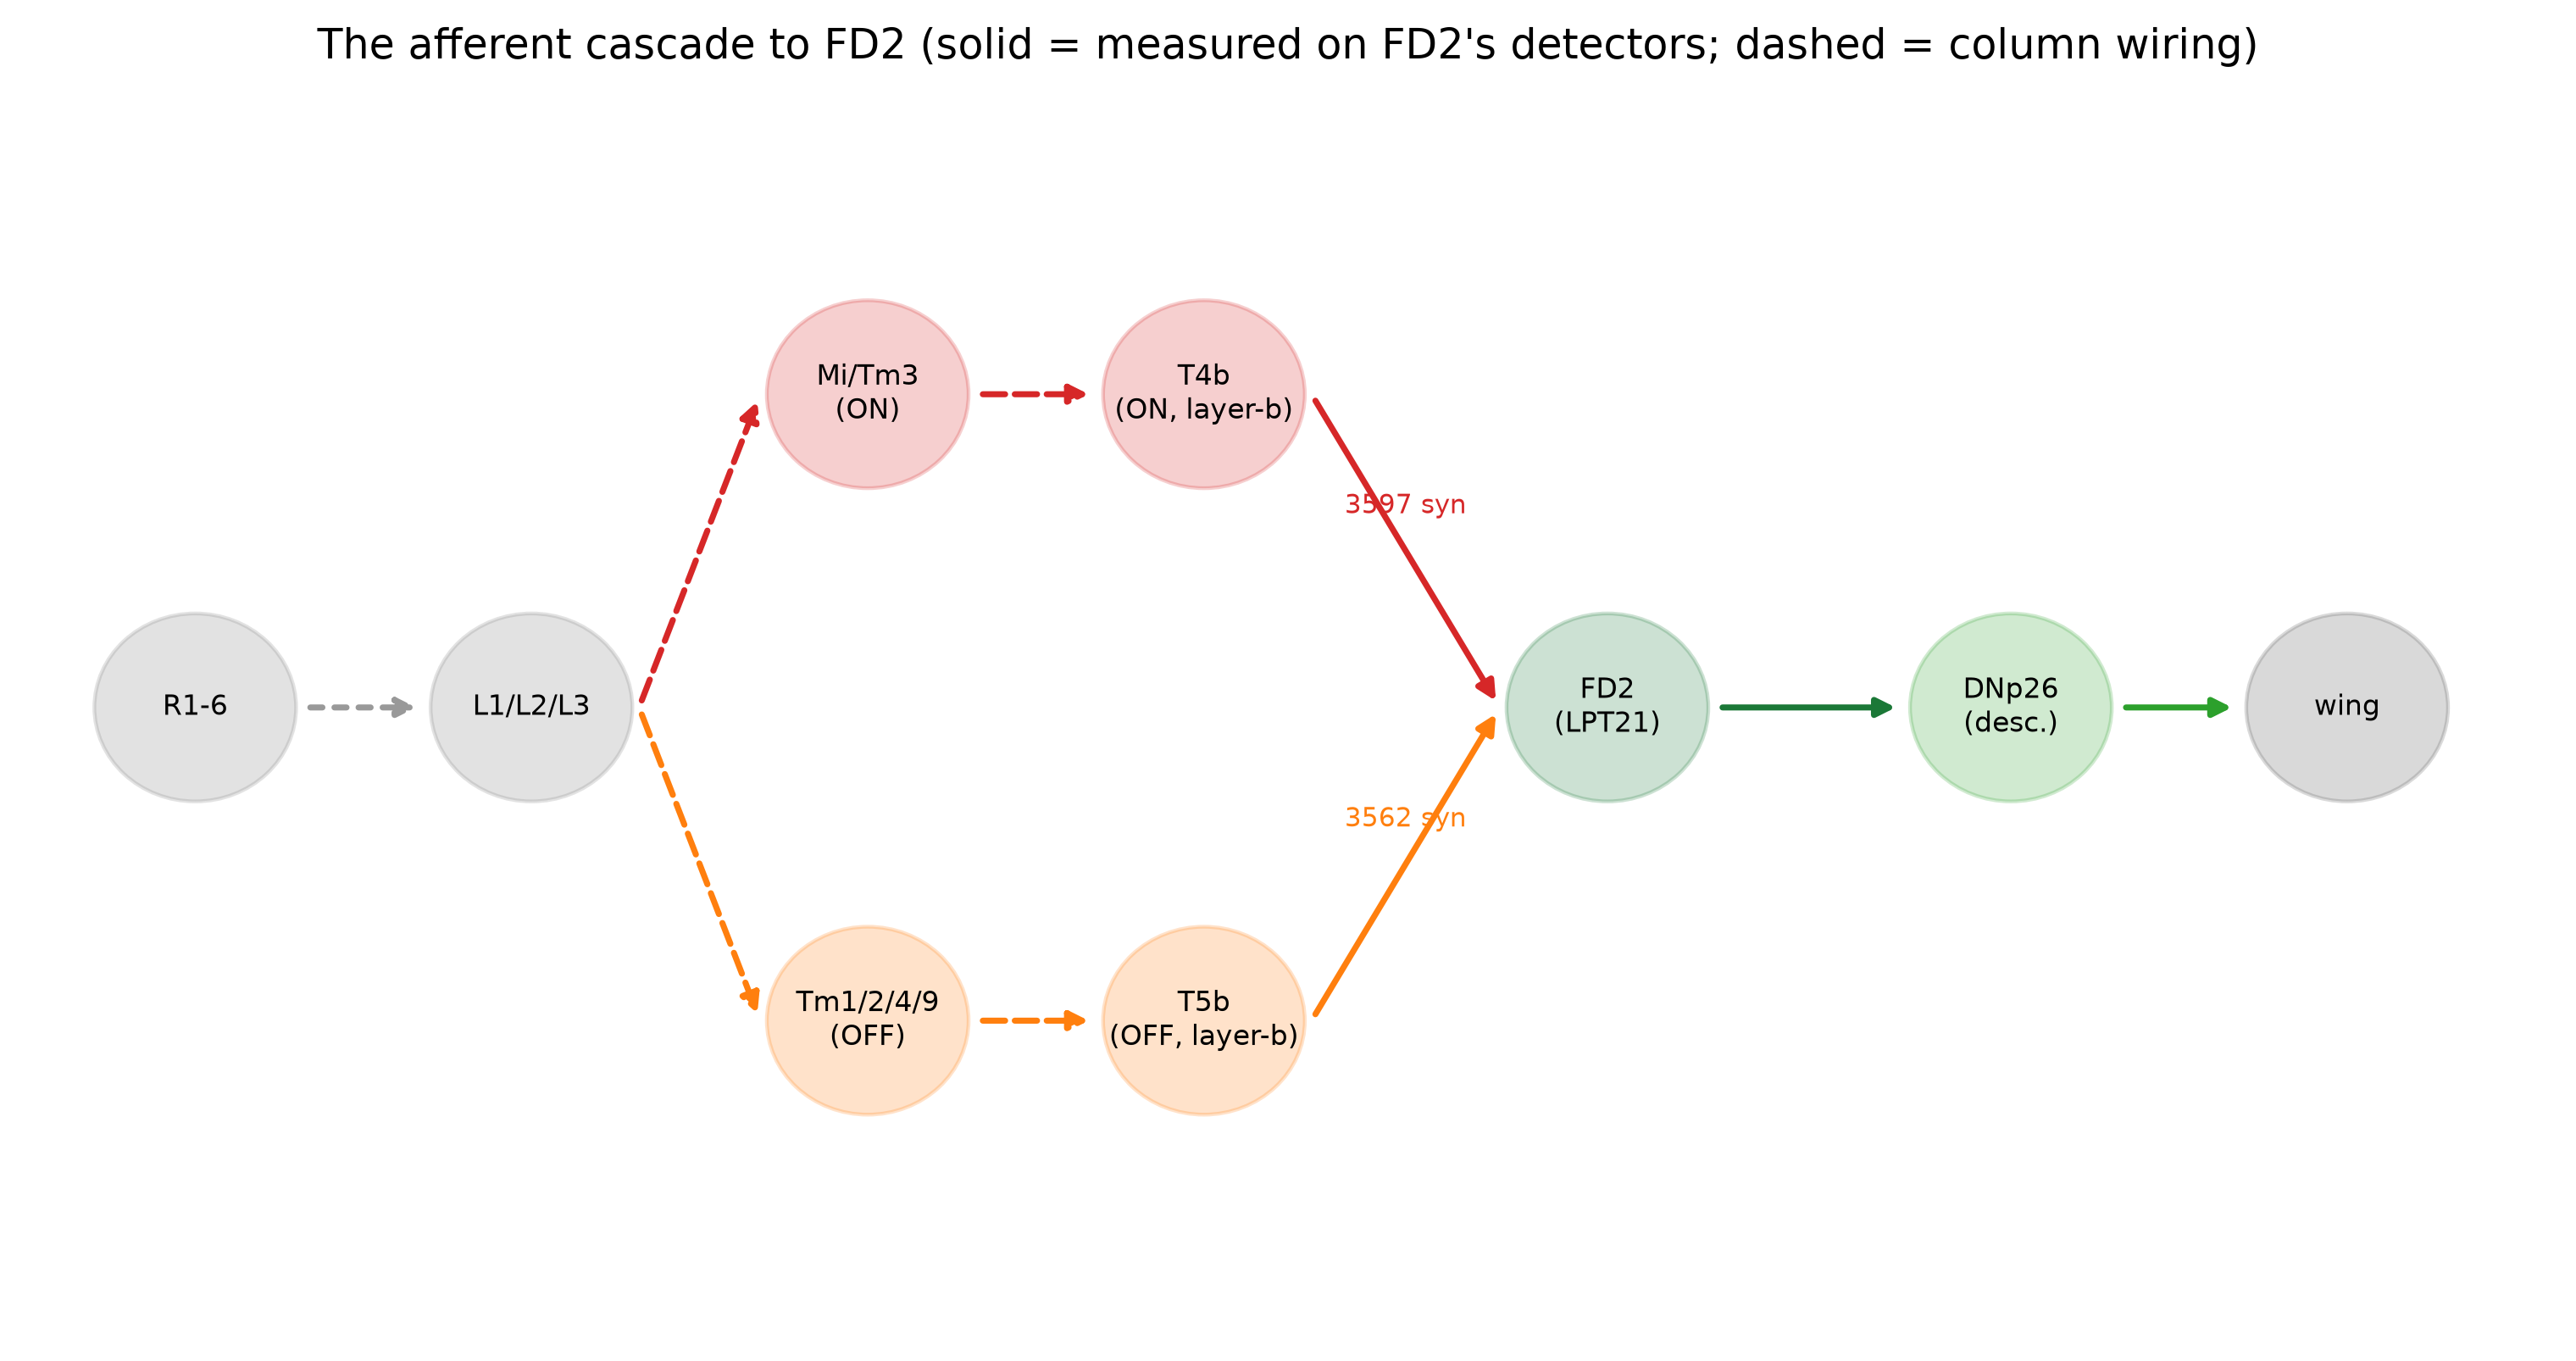
\includegraphics[width=\textwidth]{figures/fd2_afferent_cascade.png}
\caption{\textbf{The afferent cascade.} Photoreceptors to lamina to ON/OFF medulla to the back-to-front detectors \ttt{T4b}/\ttt{T5b} to FD2. Solid links are measured on FD2's detectors; dashed links are the standard column wiring.}\label{fig:cascade}
\end{figure}


\section{Where the input lands}

Each motion detector looks at one point in the eye, so the detectors feeding FD2 draw out its receptive field on the eye's lattice. Plotting those input columns shows FD2's field frontal, at the position of the FD1 cell (Fig.~\ref{fig:hexmap}).

\begin{figure}[H]\centering
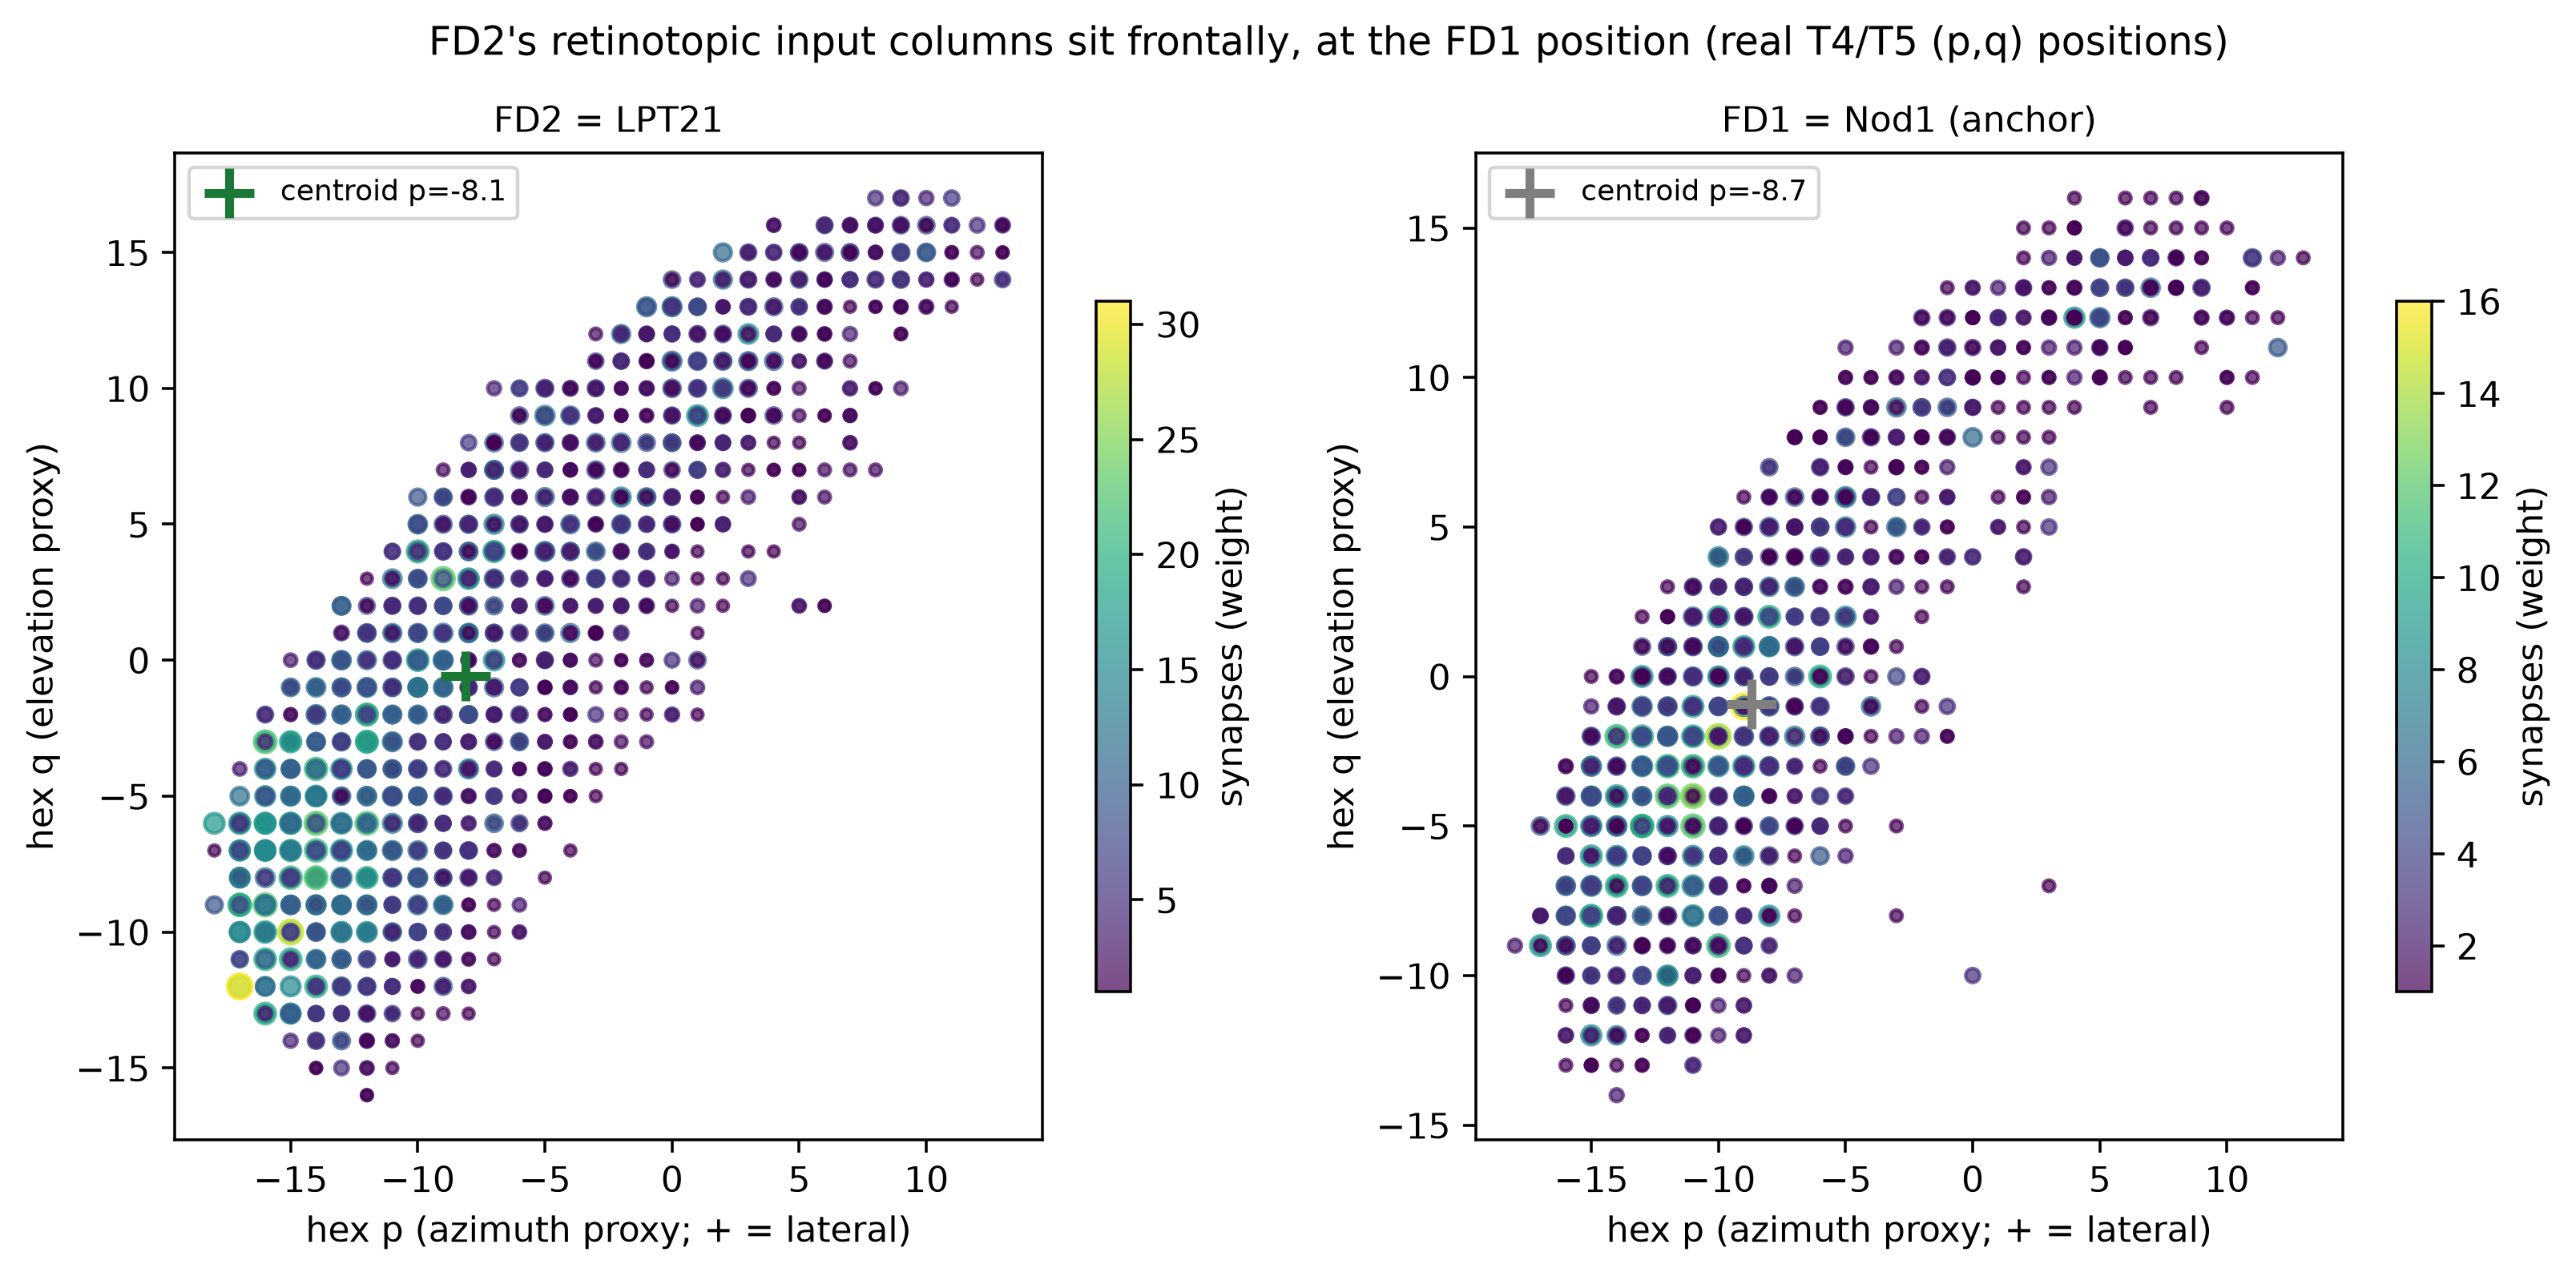
\includegraphics[width=\textwidth]{figures/fd2_input_hexmap.png}
\caption{\textbf{FD2's input in eye coordinates.} Every motion column feeding \ttt{LPT21}, placed on the eye's hexagonal lattice and shaded by synapse number, next to the frontal FD1 columns. FD2's field sits frontally, at the FD1 position.}\label{fig:hexmap}
\end{figure}


\section{The columnar sheet and the inhibitory gate}

The motion detectors also reach FD2 through a columnar projection sheet, the direction-matched layer-b sheet \ttt{LPC1}. In addition, FD2 receives input from wide-field inhibitory cells. Egelhaaf could not resolve FD2's large-field inhibitory input physiologically; the connectome resolves it as a set of lobula-plate intrinsic (\ttt{LPi}) cells, led by \ttt{LPi14}, that inhibit the cell and its detectors. The sign and function of each inhibitory partner remain wiring inferences unless supported by transmitter identity or physiology.

\begin{figure}[H]\centering
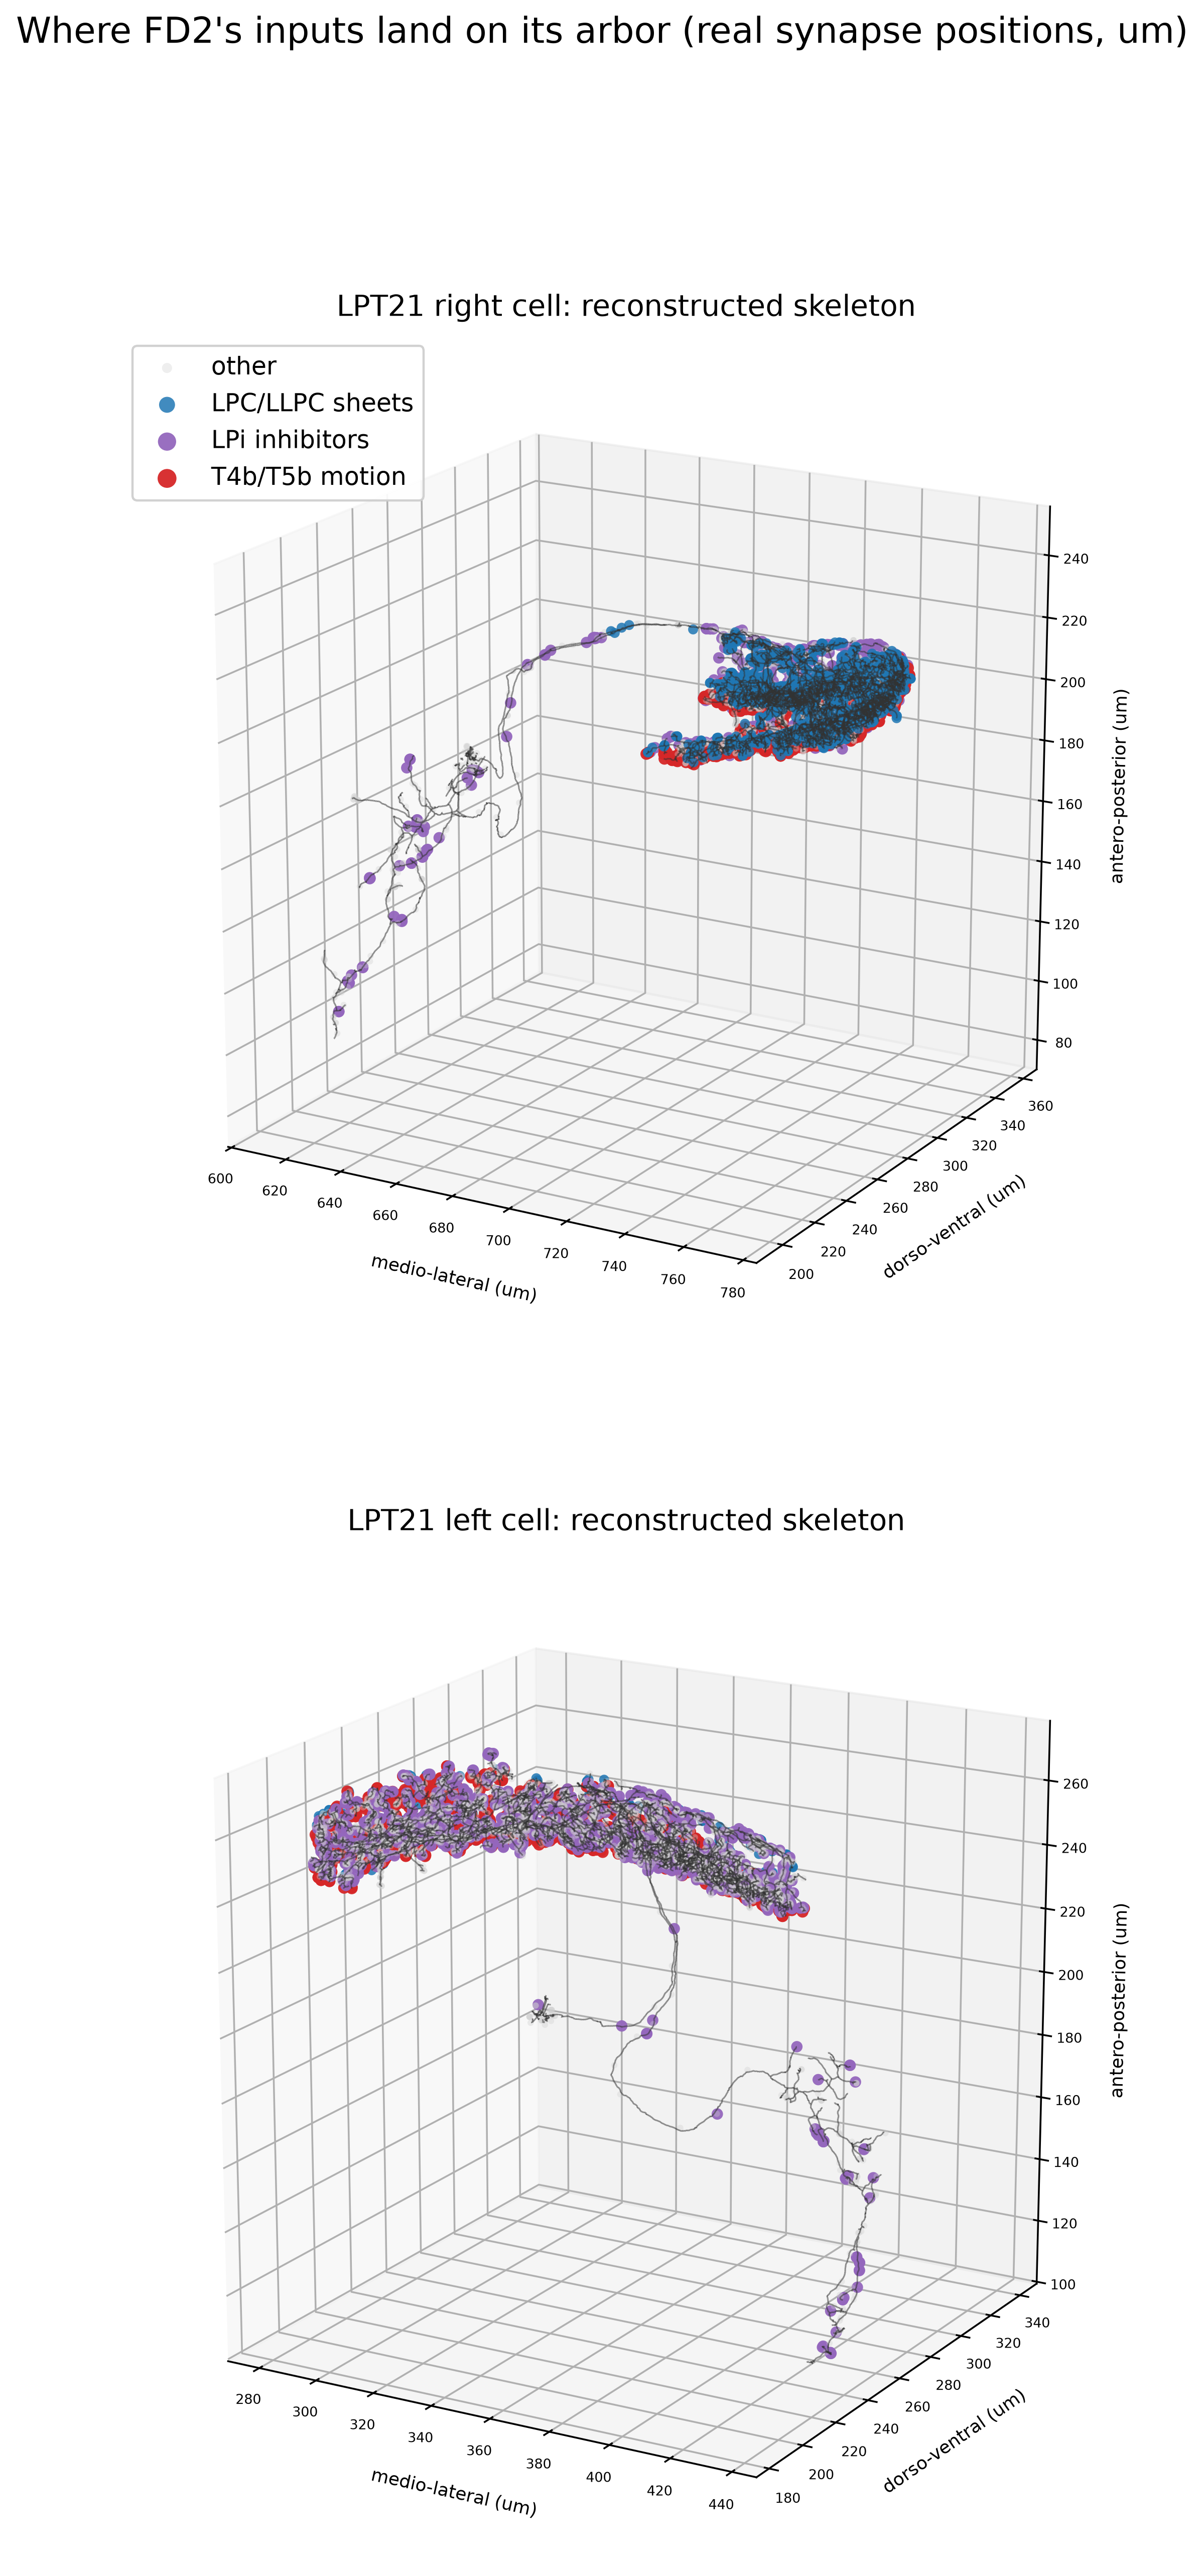
\includegraphics[width=\textwidth]{figures/fd2_arbor_inputs.png}
\caption{\textbf{Inputs on FD2's arbor.} Each \ttt{LPT21} cell's reconstructed shape with its input synapses drawn at their real positions and coloured by the class of partner: back-to-front motion detectors, columnar sheets, and inhibitory cells.}\label{fig:arbor}
\end{figure}


\section{What the data can and cannot settle}

\textbf{The upstream cascade is general wiring.} The photoreceptor-to-detector cascade is measured cell-type by cell-type across the optic lobe and matches the known column wiring; it is shown as the pathway culminating in FD2's detectors, not as an FD2-specific trace. \textbf{The inhibitory gate is a wiring inference.} That the resolved \ttt{LPi} partners are inhibitory follows from their transmitter, but the direction and functional role of the gate are inferences the connectome sets up rather than measures.

\clearpage

\part{Outputs: descending and motor-system partners}

\textbf{Summary.}\quad For FD2's figure signal to influence movement it must reach descending neurons, which project from the brain into the ventral nerve cord and contact motor-control networks. \ttt{LPT21} contacts descending neurons directly, led by \ttt{DNp26}, and its descending output is biased toward the wing-steering motor system when each descending neuron is followed into the male nerve-cord connectome.

\section{The descending neurons FD2 contacts directly}

\ttt{LPT21} makes 122 output synapses onto 8 descending-neuron types. The leading target is \ttt{DNp26}, the same wing-steering command neuron that the FD1 and FD3 arms reach, so the three figure cells converge on a shared descending target (Fig.~\ref{fig:dnrank}). Egelhaaf could name only ``descending neurones'' generically; the connectome names them.

\begin{figure}[H]\centering
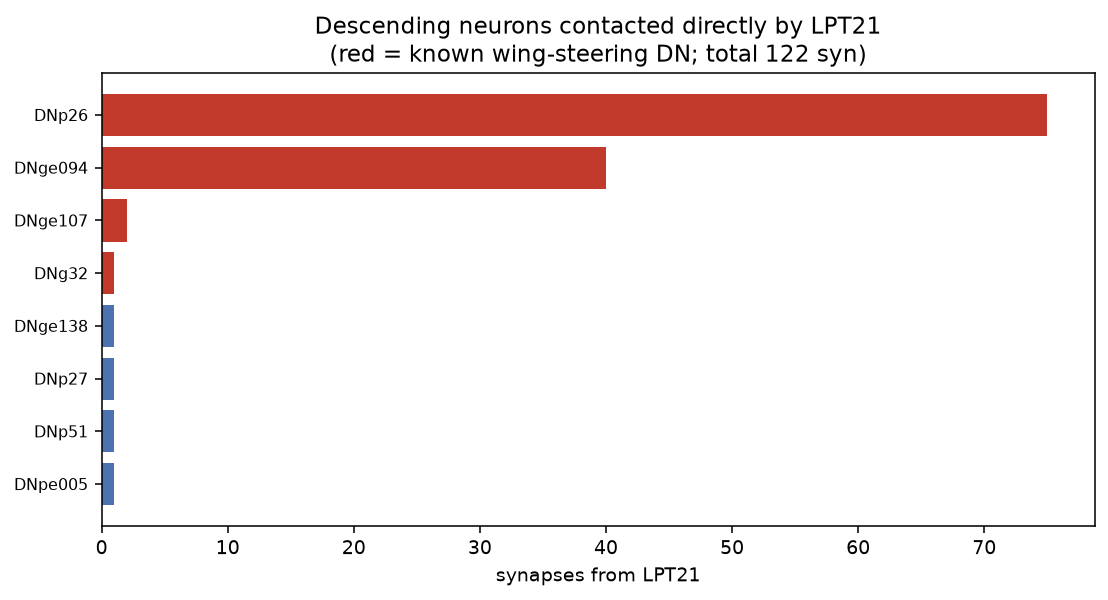
\includegraphics[width=\textwidth]{figures/fd2_dn_ranking.png}
\caption{\textbf{The descending neurons FD2 contacts directly.} Each bar is one descending-neuron type, ranked by synapses received from \ttt{LPT21}. Red marks neurons known to drive wing-steering muscles.}\label{fig:dnrank}
\end{figure}


\section{Motor systems contacted by those neurons}

Classifying the descending neurons FD2 reaches by whether they are known wing-steering command neurons, the great majority of FD2's descending output goes to that class (dominant system: \ttt{wing\_steering}; Fig.~\ref{fig:motorsys}). The principal target \ttt{DNp26} drives the contralateral wing-steering muscles in the male nerve-cord connectome. Two qualifications keep this precise. First, the class label is by descending-neuron identity, not by muscle count: when each descending neuron is followed into the male nerve cord and weighted by its actual motor targets, the leading neuron \ttt{DNp26} splits its output between wing-steering and neck muscles, and the second target is neck and abdominal rather than wing, so the honest picture is a bias toward steering and gaze control rather than pure wing steering. Second, the descending contact is sparse (of the order of a hundred synapses), most of it carried by the top two neurons. The pathway therefore supports a steering and gaze-control role, consistent with Egelhaaf's proposal that the FD cells contribute to yaw-torque control, but it does not by itself prove that FD2 activity drives a behaviour.

\begin{figure}[H]\centering
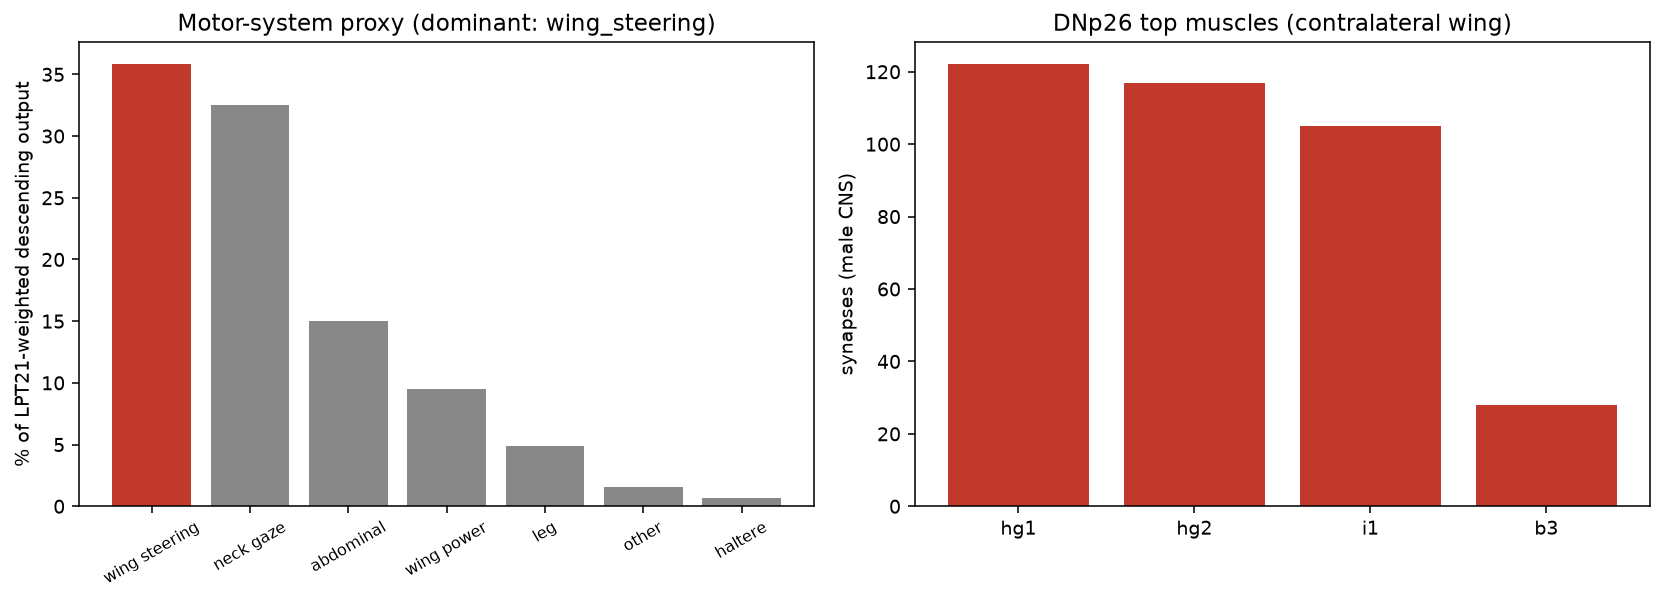
\includegraphics[width=\textwidth]{figures/fd2_motor_systems.png}
\caption{\textbf{Motor-system proxy.} (left) The motor systems reached by FD2's descending output, weighted by how strongly FD2 drives each descending neuron and classified by descending-neuron identity; the wing-steering class has the largest share, though weighting by actual muscle targets softens this toward a mixed steering and neck-gaze bias (see caveats). (right) The top wing-steering muscles of the principal descending target in the male nerve-cord connectome.}\label{fig:motorsys}
\end{figure}


\section{The circuit in the brain}

Seen alongside the cells it connects, FD2 sits anatomically between the lobula-plate motion detectors and the descending neurons that contact wing-steering motor systems (Fig.~\ref{fig:circuit3d}).

\begin{figure}[H]\centering
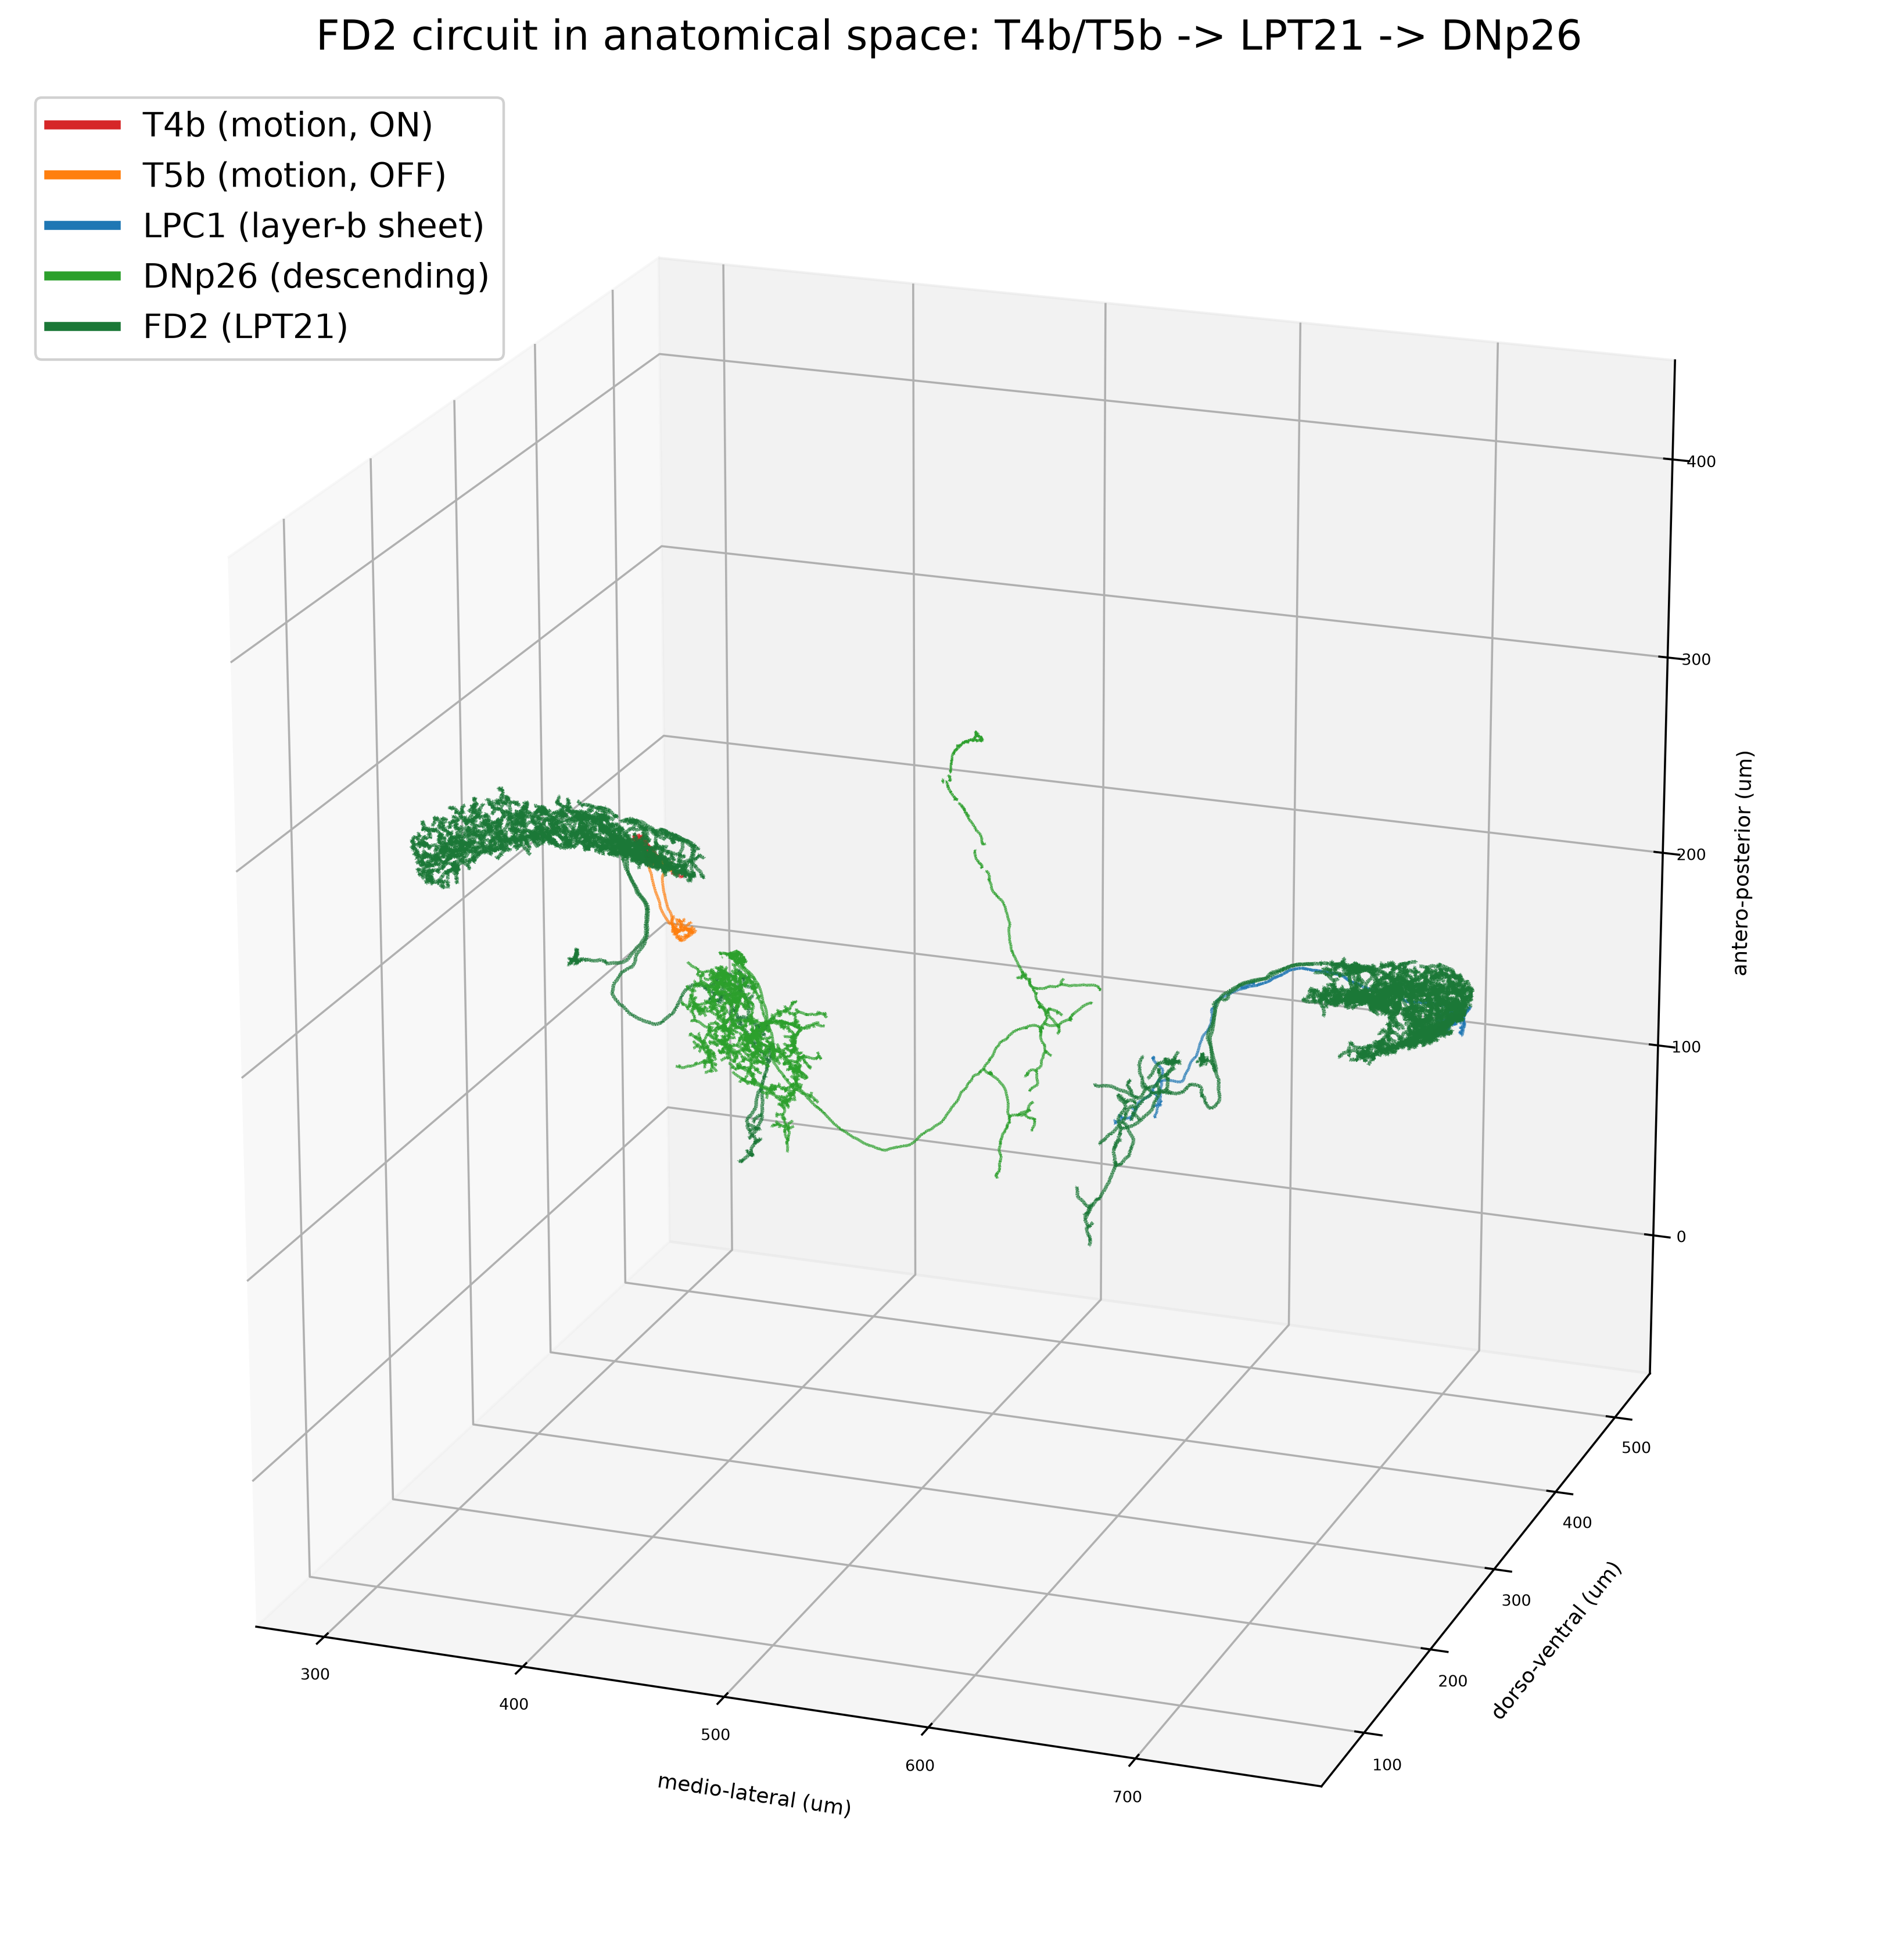
\includegraphics[width=\textwidth]{figures/fd2_circuit_3d.png}
\caption{\textbf{The circuit in the brain.} Reconstructed neurons of the FD2 pathway in their true anatomical positions: the \ttt{T4b}/\ttt{T5b} motion detectors, both \ttt{LPT21} cells, and the descending neuron they lead to.}\label{fig:circuit3d}
\end{figure}


\section{What the data can and cannot settle}

\textbf{The steering label is by neuron identity, not muscle count.} The wing-steering share reported above counts descending neurons that belong to the known wing-steering set; weighting instead by each neuron's actual motor targets in the male nerve cord softens the picture to a mixed wing-steering and neck-gaze bias, because the leading descending neuron contacts neck as well as wing muscles and the second target is neck and abdominal. The direction of the bias (toward steering and gaze control) is robust; its exact magnitude depends on which of the two weightings is used. \textbf{The muscle map crosses two connectomes.} The muscles each descending neuron drives are read from a second, male nerve-cord connectome, bridged to the brain by the shared descending-neuron name; a neuron without a named counterpart contributes no muscle information. \textbf{The descending contact is sparse.} FD2's direct descending output is of the order of a hundred synapses, most of it onto the top two neurons, so the read-out rests on a small number of strong contacts rather than a broad projection. \textbf{FD2 is two cells.} The result rests on the two cells agreeing, not on a population average.

\clearpage

\part{The functional figure-ground circuit of FD2}

\textbf{Summary.}\quad This part maps FD2's whole connectivity and then names the working figure-ground circuit within it, in the same terms as the FD1 and FD3 arms: motion detectors to the layer-b sheet \ttt{LPC1} to FD2 to the steering neuron \ttt{DNp26}, gated by the wide-field inhibitor \ttt{LPi14}.

\section{FD2's connectivity, comprehensively}

\ttt{LPT21} receives about 18822 input synapses from roughly 3771 partner cells, and makes about 26071 output synapses onto roughly 12323 partners. The inputs are dominated by the motion detectors, the neighbouring columnar sheets, and inhibitory cells; the outputs are broadcast to central brain cells and, through the descending neurons, toward the steering muscles (Fig.~\ref{fig:wheel}).

\begin{figure}[H]\centering
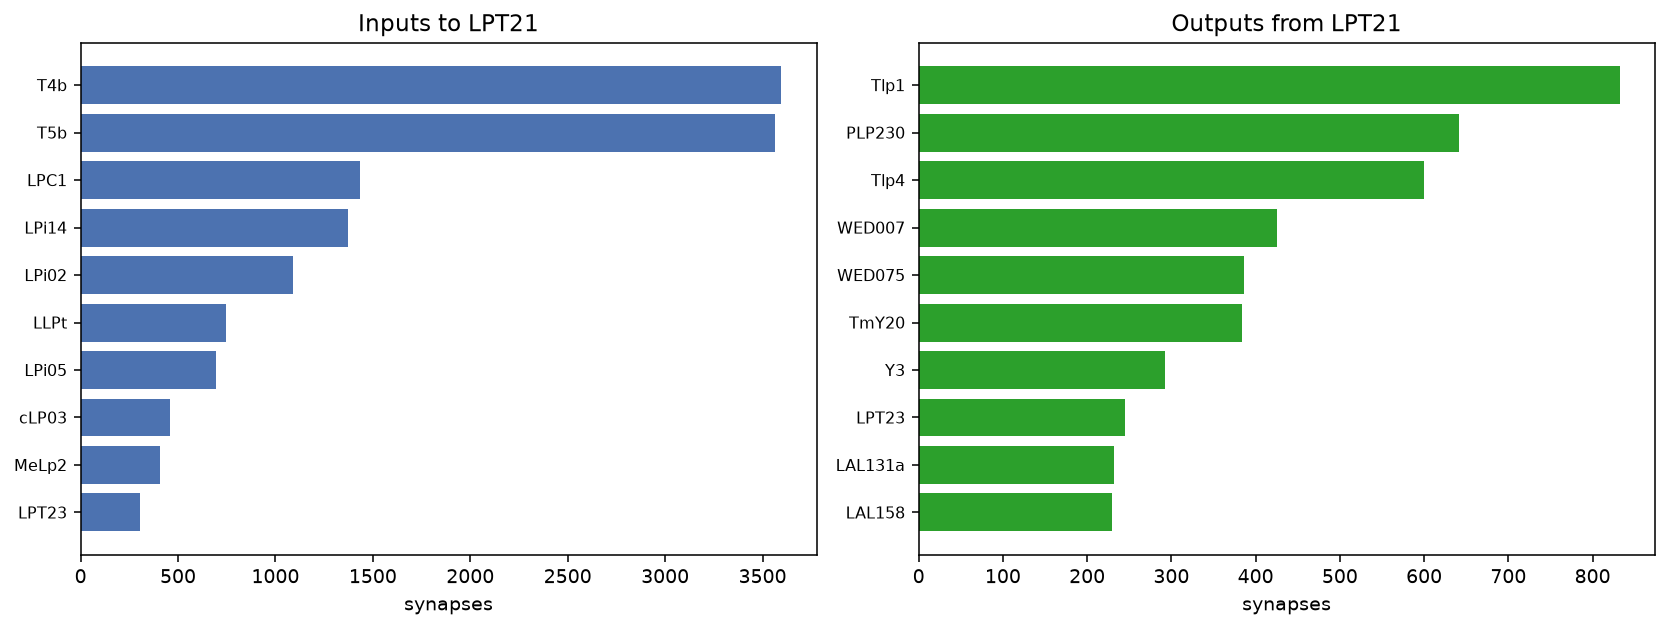
\includegraphics[width=\textwidth]{figures/fd2_connectivity_wheel.png}
\caption{\textbf{FD2's comprehensive connectivity.} Every major input (left) and output (right) partner type of \ttt{LPT21}.}\label{fig:wheel}
\end{figure}


\section{Where inputs land}

Splitting FD2's input synapses between its dendrite and its axon shows that the input arrives on the dendritic arbour in the lobula plate, while the axon carries the cell's output. FD2 is thus a cleanly polarised neuron (Fig.~\ref{fig:compartment}).

\begin{figure}[H]\centering
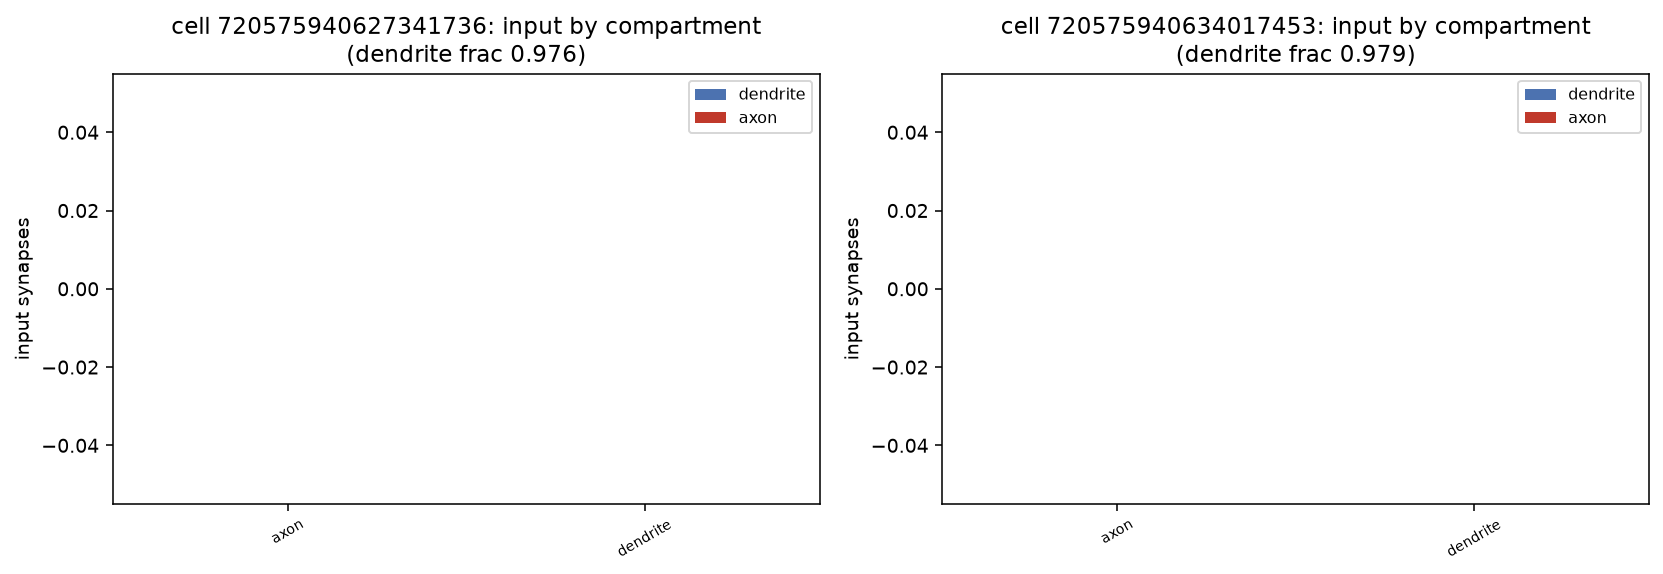
\includegraphics[width=\textwidth]{figures/fd2_compartment_split.png}
\caption{\textbf{Where inputs land.} Input synapses to each \ttt{LPT21} cell, split between the dendrite and the axon and coloured by the class of partner.}\label{fig:compartment}
\end{figure}


\section{The circuit, named end to end}

Putting the pieces together, FD2's figure-ground circuit reads: the \ttt{T4b}/\ttt{T5b} back-to-front motion detectors drive the layer-b sheet \ttt{LPC1}, which relays to FD2; FD2 drives the steering command neuron \ttt{DNp26} and thence the wing; and the wide-field cell \ttt{LPi14} gates the circuit. This is the same architecture as the FD1 and FD3 arms, built from a frontal, regressive, homolaterally projecting cell, and it terminates on the shared wing-steering command neuron. Whether the frontal branch additionally serves the landing response, as Egelhaaf proposed, is a question the wiring sets up but does not answer.

\begin{figure}[H]\centering
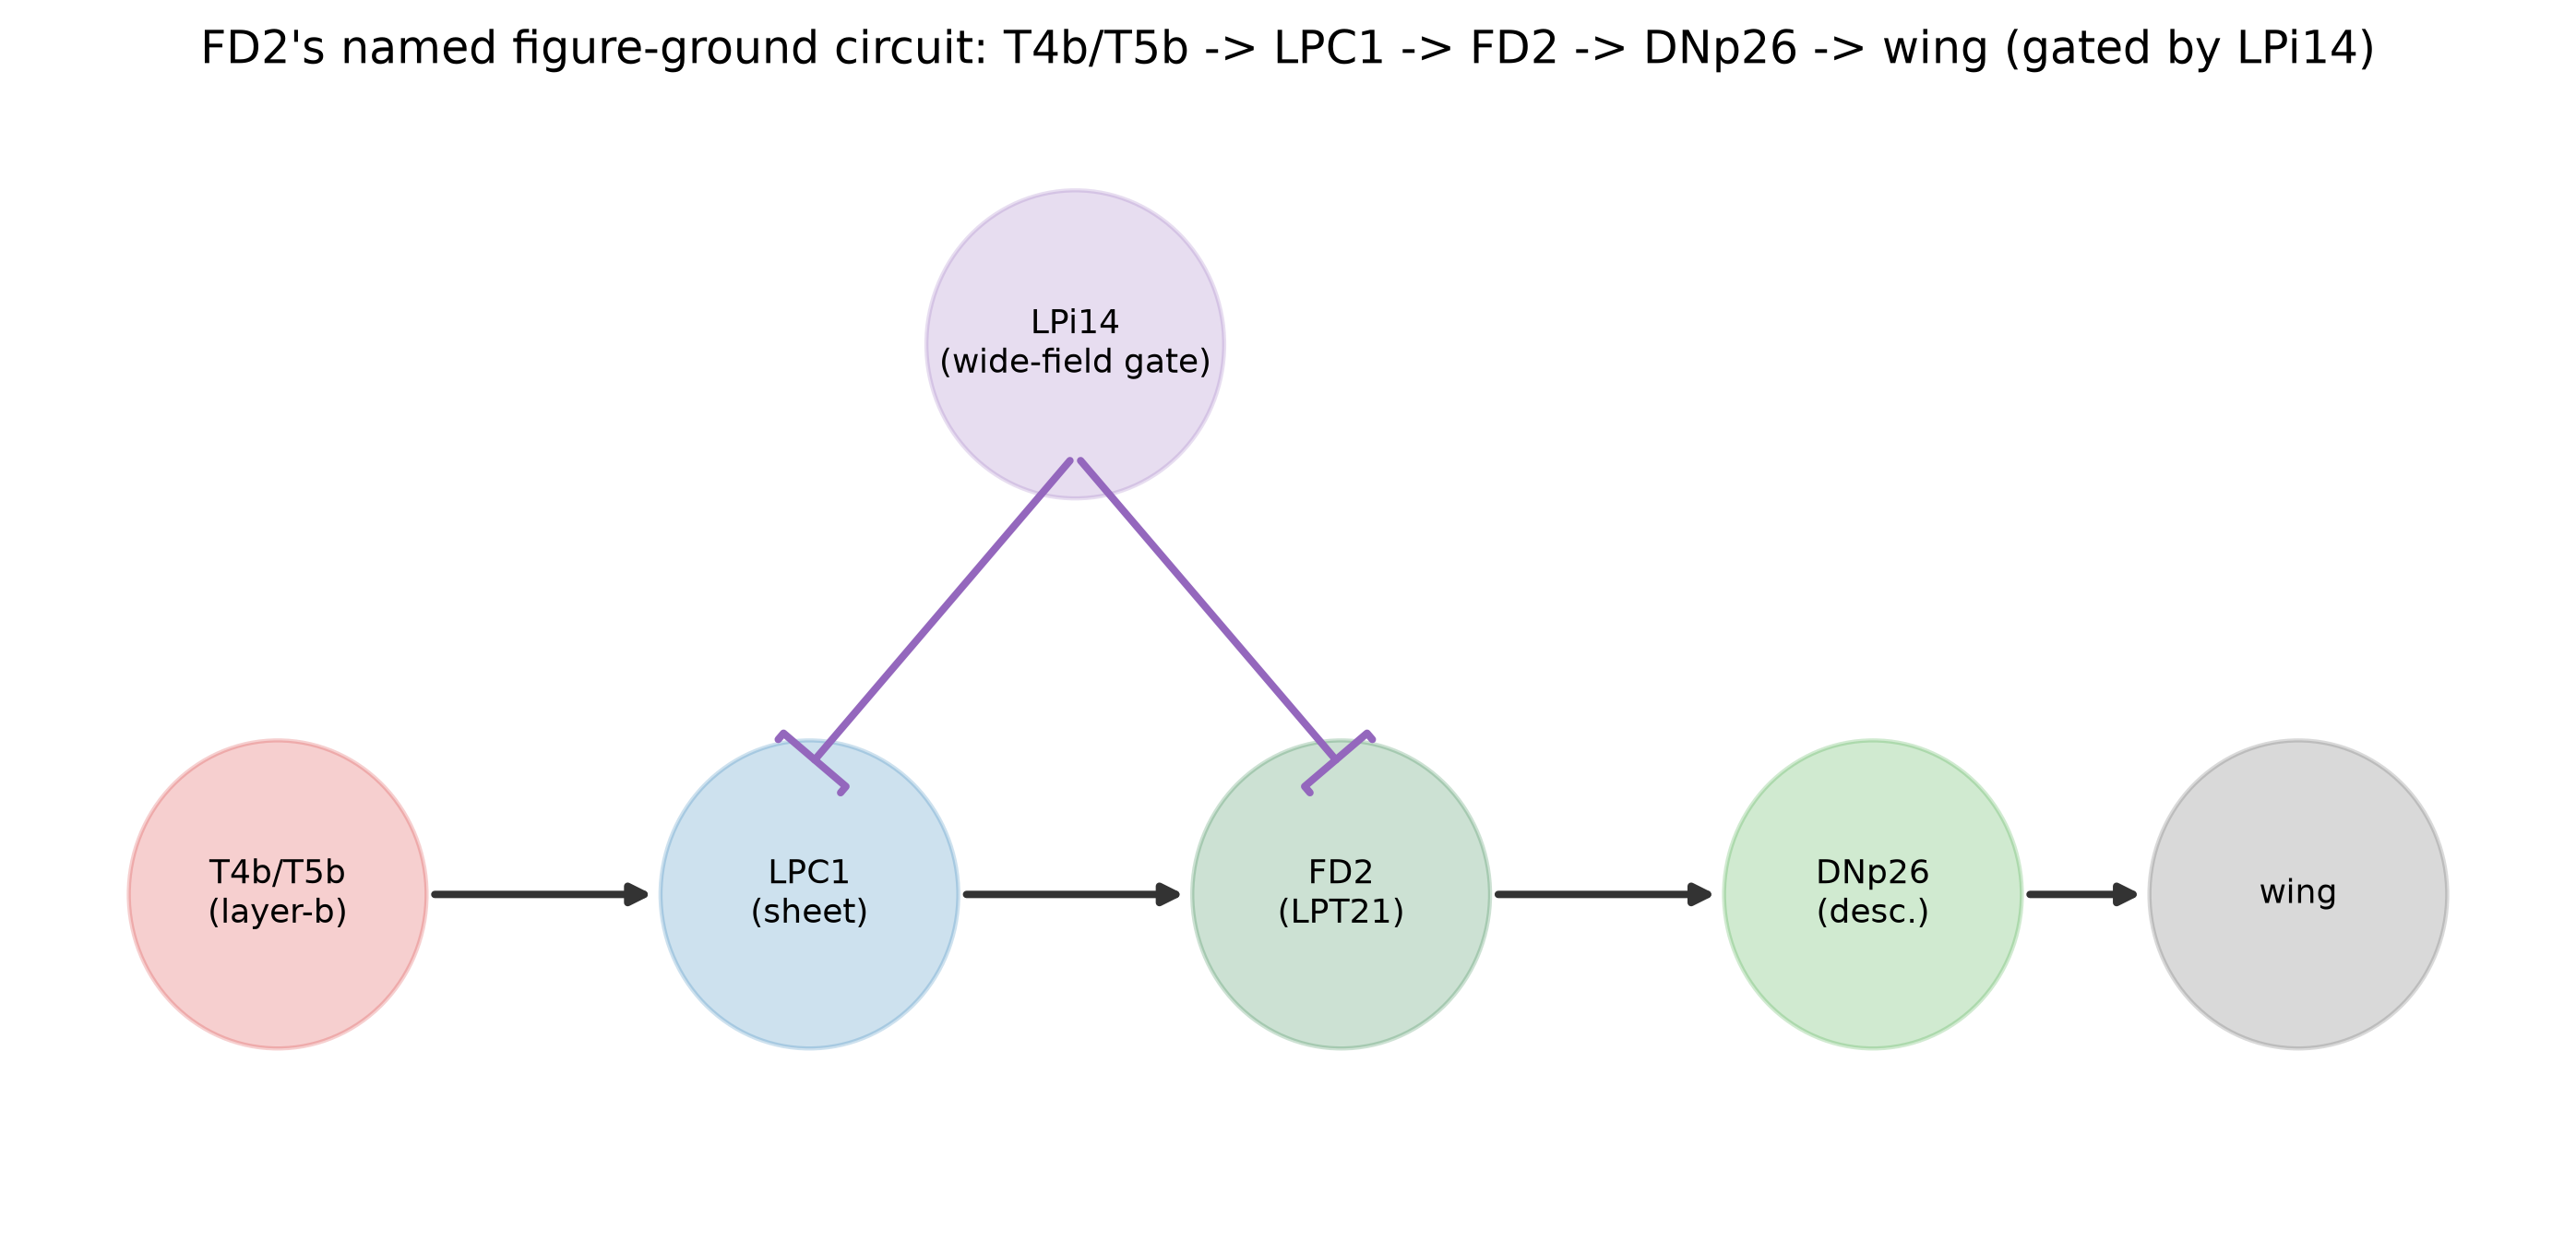
\includegraphics[width=\textwidth]{figures/fd2_functional_circuit.png}
\caption{\textbf{The named figure-ground circuit.} \ttt{T4b}/\ttt{T5b} motion detectors drive the layer-b sheet, which relays to FD2; FD2 drives the steering neuron and the wing, with a wide-field inhibitory gate. Numbers are measured synapse counts.}\label{fig:funcircuit}
\end{figure}


\section{What the data can and cannot settle}

\textbf{Sign is not read from wiring.} That a GABAergic contact is inhibitory, and that the gate shapes FD2's figure response, are expectations from physiology; the connectome supplies the connections, not the sign or the response. \textbf{The landing-response role is a hypothesis.} Egelhaaf proposed that FD2's frontal branch drives the landing response; the connectome confirms the dual output but does not measure the behaviour. \textbf{FD2 is one bilateral pair.} As throughout, the result rests on the two cells agreeing and on the thousands of synapses each makes.

\section{Methods and provenance}

\textbf{Connectome.} FlyWire FAFB materialization v783 (\ttt{synapses\_nt\_v1}, no cleft threshold), track \ttt{live}, with the homolateral (contra\%) identity measurement confirmed across the offline, live and v630 tracks. Neuron annotations are the Schlegel/Codex tables. \textbf{Preferred direction} is the synapse-weighted T4/T5 lobula-plate layer composition~\cite{fd1989,maisak2013}. \textbf{Receptive field}: T4/T5 inputs carry hex-lattice coordinates; the differential test compares the synapse-weighted centroid and frontal-band occupancy against the FD1=\ttt{Nod1} anchor with a within-cell bootstrap, the axis pinned by requiring the known-frontal FD1 anchor to land frontal. \textbf{Projection side} is the fraction of output synapses on the contralateral side. \textbf{Dual output} is a bimodality test on each cell's output-synapse field. \textbf{Uniqueness} scans the lobula-plate tangential family for the FD2 conjunction. \textbf{Afferent, sheet, gate, efferent} reuse the FD-circuit machinery parameterised on \ttt{LPT21}; the motor read-out crosses into the male CNS by shared descending-neuron name. \textbf{Reproducibility}: built from the FD2 verification JSON.

\clearpage

\begin{thebibliography}{11}
\bibitem{egelhaaf1985a} Egelhaaf M. (1985) On the neuronal basis of figure-ground discrimination by relative motion in the visual system of the fly. I. \textit{Biol. Cybern.} 52:123--140.
\bibitem{egelhaaf1985b} Egelhaaf M. (1985) \ldots II. Figure-detection cells, a new class of visual interneurones. \textit{Biol. Cybern.} 52:195--209. (FD2 at pp.~201--202, 207--208.)
\bibitem{egelhaaf1985c} Egelhaaf M. (1985) \ldots III. Possible input circuitries and behavioural significance of the FD-cells. \textit{Biol. Cybern.} 52:267--280.
\bibitem{rp1979} Reichardt W., Poggio T. (1979) Figure-ground discrimination by relative movement in the visual system of the fly. I. \textit{Biol. Cybern.} 35:81--100.
\bibitem{fd1989} Fischbach K.-F., Dittrich A.P.M. (1989) The optic lobe of \textit{Drosophila melanogaster}. I. A Golgi analysis of wild-type structure. \textit{Cell Tissue Res.} 258:441--475.
\bibitem{maisak2013} Maisak M.S. et al. (2013) A directional tuning map of \textit{Drosophila} elementary motion detectors. \textit{Nature} 500:212--216.
\bibitem{namiki2018} Namiki S. et al. (2018) The functional organization of descending sensory-motor pathways in \textit{Drosophila}. \textit{eLife} 7:e34272.
\bibitem{dorkenwald2024} Dorkenwald S. et al. (2024) Neuronal wiring diagram of an adult brain. \textit{Nature} 634:124--138.
\bibitem{schlegel2024} Schlegel P. et al. (2024) Whole-brain annotation and multi-connectome cell typing of \textit{Drosophila}. \textit{Nature} 634:139--152.
\bibitem{codex} FlyWire Codex, \texttt{codex.flywire.ai} -- cell-type and annotation portal.
\end{thebibliography}

\end{document}